\chapter{H$_{2}$O in an external electric dc field}
\label{ch:dc_h2o}

% H2O in strong dc fields
% effective potential
% outline of the chapter


The Stark resonance parameters, which characterize the shift and decay
width of the molecular energy levels under an external dc field, are
fundamental in the study of the strong dc field ionization of
molecular orbitals (\textsc{mo}s). In the case of the water molecule,
the multicentre nature of the combined Coulomb interactions and,
consequently, the additional degrees of freedom, make the strong dc
field ionization of H$_{2}$O an attractive and challenging problem
from the point of view of a theoretical description.
%as well as
%experimentally. % refs [14-17 pra]
Complex variable techniques, such as exterior complex scaling
(\textsc{ecs})~\cite{Simon_1979,ecsScrinzi} and complex-absorbing
potentials (\textsc{cap})~\cite{RissMeyer_1993,Krause_2014}, have been
implemented in order to address the problem of molecular static-field
ionization and compute the induced Stark resonances.

The dc Stark problem for the H$_{2}$O valence orbitals is addressed in
this chapter within the framework of non-Hermitian quantum
mechanics~\cite{Moiseyev_NHQM}. Two independent complex variable
techniques are implemented in order to modify the divergent outgoing
wave functions into the physical domain of square integrable wave
functions. A modified \textsc{ecs}, in which the Hamiltonian of the
system is gradually rotated into the complex plane to obtain the
resonance parameters induced by an external dc field, is the first of
these approaches. The construction of a local effective potential,
which reflects the individual properties of the orbitals, is crucial
in this study. An alternative analysis is based on a quadratic
\textsc{cap} which requires successive calculations of complex
eigenvalues along a trajectory that is determined by the strength
parameter of the \textsc{cap}. The \textsc{cap} method is then
combined with a correction scheme in order to eliminate the artifact
introduced in the Hamiltonian by the complex absorber.

Section~\ref{ch:nonH_qm} introduces some of the fundamental aspects of
non-Hermitian quantum mechanics. In Sec.~\ref{ch:h2o_structure}, we
formulate the problem with emphasis on the representation of the
molecular orbitals. The \textsc{ecs} formalism is introduced in
Secs.~\ref{ch:1b1_1b2} and~\ref{ch:3a1} as a crucial step in finding a
numerical solution to a spherically symmetric problem, in the case of
the $1b_{1}$ and $1b_{2}$ orbitals, and the problem of a non-central
effective potential, in the case of the $3a_{1}$
orbital. Section~\ref{ch:partial_wave} is concerned with the
discussion of a partial-wave expansion method implemented for a model
potential designed to simulate the structure of the H$_{2}$O
molecule. The problem of dc-ionization of the H$_{2}$O valence
orbitals is treated in terms of a \textsc{cap}. The Stark resonance
parameters are then presented in Sec.~\ref{ch:stark_params}, in which
the symmetry properties of the orbitals are considered
independently. The analysis presented in this chapter compiles that
of~\cite{sarias_2016,sarias_2017}.


\section{Non-Hermitian quantum mechanics}
\label{ch:nonH_qm}
% introduction of the basic principles of this formulation of QM
% introduce complex-variable methods used later on: ECS and CAP

Resonance phenomena, such as atomic and molecular strong-field
ionization events, have been successfully approached within the
framework of non-Hermitian quantum
mechanics~(\textsc{nhqm})~\cite{Moiseyev_NHQM}. This alternative
formulation to the standard formalism of quantum mechanics allows for
a time-independent interpretation of strong-field ionization processes
and quantitative modelling of the associated ionization rates. This is
possible by means of implementing analytic continuation methods on the
Hamiltonian, from which the resonance is obtained as a solution with
complex eigenvalues of the form
%
\begin{eqnarray}
  E = E_{R} + i E_{I} = E_{R} - i \Gamma/2,
  \label{eq:complex_eigenE}
\end{eqnarray}
%
in which the ionization rate, $\Gamma$, induced by the external field
$F_{0}$ is associated to the lifetime of the decaying state $\tau$ via
$\Gamma\tau = 1$, while the real part $E_{R}$ represents the Stark
shift under the external field.

Several numerical techniques have been introduced within the framework
of \textsc{nhqm} that implement a complex-scaled Hamiltonian in
studies of atomic and molecular Stark resonances. It is the scope of
this work to focus on two of these methods to study the response of
the H$_{2}$O highest-energy orbitals to an external dc-field, the
concept of a \textsc{cap} introduced as a perturbation to the
molecular Hamiltonian and a modified \textsc{ecs}.

% add artificial potential introduced to absorb outgoing wave

% relevant parameters in a CAP (equation for the CAP used in the
% partial wave calculations)

% approach to obtain the resonances (to remove the perturbation
% introduced by the CAP)

A \textsc{cap} is introduced as an imaginary potential which
introduces an analytical continuation of the Hamiltonian to the
complex plane. This artificial perturbation of the system acts as an
effective absorber potential that suppresses the diverging tail of the
resonance wave function in the vicinity of the edges of a numerical
grid. As a result, the solutions of the modified non-Hermitian
Hamiltonian behave as square-integrable eigenstates.
%within the original boundary conditions.

In general terms, the application of a \textsc{cap} begins with the
addition of an artificial local potential of the form $-i \eta W(r)$
to the Hamiltonian of the system, where the parameter $\eta$ indicates
the strength of the \textsc{cap}. The function $W(r)$, which
determines the onset of the \textsc{cap}, has been most commonly
defined as a quadratic potential centred at some radius
$r_{\mathrm{c}}$.%add refs?
The \textsc{cap} approach requires calculating sets
of complex eigenvalues along complex trajectories, $E(\eta)$,
determined by the \textsc{cap} strength in order to find an optimal
finite value of $\eta$ such that it makes the resonance stable, with
the ultimate goal of removing the perturbation by the \textsc{cap}.

Strategies used to obtain the optimal value of $\eta$ include the
Pad\'{e}-approximation-extrapolation
procedure~\cite{Moiseyev_Pade_2005}, and the Riss-Meyer iterative
correction method~\cite{RissMeyer_1993}. Combining such correction
schemes with a \textsc{cap} has proven to yield accurate results for
the Stark resonance parameters of diatomic molecules, such as the
hydrogen molecular ion in a static electric field~\cite{Tsog_2013} and
a low-frequency ac field~\cite{Tsog_H2mol_ac_2013}.
% add references cited in the partial wave write-up and Moiseyev book on NHQM

An alternative method to divert the divergent resonance wave functions
into the physical domain of square integrable solutions is the
\textsc{ecs}~\cite{Simon_1979}, in which one or more coordinates are
rotated into the complex plane at a boundary of the problem. The
application of the complex scaling in an external region, which keeps
the coordinates unscaled in some range of the potential, avoids the
numerical difficulties that arise when the potential has
singularities. This approach, however, imposes explicit discontinuity
conditions on the wave function and its
derivatives~\cite{ScrinziJChemPhys_ECS}. The method of \textsc{ecs}
has proven to be useful in acting as a perfect absorber of the
outgoing flux when solving the \textsc{tdse} with strong laser
fields~\cite{ecsScrinzi}. The implementation of a smooth \textsc{ecs}
to the radial coordinates of an orbital-dependent Hamiltonian that
represents the H$_{2}$O valence orbitals is one of the motivations of
the current chapter.

% MENTION THAT ECS AND CAP ARE EQUIVALENT IN SOME WAY 


\section{Molecular orbital representation of H$_{2}$O}
\label{ch:h2o_structure}
% Formulation of the Problem

The starting point for this study is the Hartree-Fock (\textsc{hf})
calculation of the H$_{2}$O molecular states using a single-center
Slater orbital
basis~\cite{Moccia_1964,Moccia_JCP_2164,Moccia_JCP_2176}, applied to
collision studies~\cite{Montanari_2013} and compared to experimental
electron spectroscopy~\cite{Hafied_2007}. Accurate descriptions of the
molecular structure of H$_{2}$O, and other diatomic molecules, have
been obtained by means of the variational Hartree-Fock method using
multicentre Slater orbitals as basis
functions~\cite{Pitzer_1968,Pitzer_1970}. However, the direct
application of these multicentre orbitals for strong-field studies
implies significant computational and methodological challenges.

The present work is intended to study the valence molecular orbitals
of H$_{2}$O, $1b_{1}$, $1b_{2}$ and $3a_{1}$. The wave functions for
the $1b_{1}$ and $1b_{2}$ molecular orbitals, which can be
approximated as the $2p_{x}$ and $2p_{y}$ oxygen orbitals, are
dominated by a single angular mometum symmetry. The $3a_{1}$
\textsc{mo}, on the other hand, consists mainly of the oxygen $2s$ and
$2p_{z}$ and the hydrogen $1s$ atomic orbitals.

The general expression for the basis functions, introduced as a set of
single-center wave
functions~\cite{Moccia_1964,Moccia_JCP_2164,Moccia_JCP_2176}, is a
Slater-type orbital as defined in Eq.~(\ref{eq:f_STO}). The expansion
coefficients and nonlinear coeficients $\{\zeta_{i}\}$, determined by
Roothaan's self-consistent-field
method~\cite{Moccia_1964,Roothaan_1951} introduced in
Sec.~\ref{ch:scf_sto}, are used to construct a reduced form of the
radial functions that describe all the molecular orbitals. More
specifically, we are interested in using a reduced \textsc{sto}
expansion to construct an effective potential that describes an
H$_{2}$O bound state as a first step in studying the response of the
H$_{2}$O valence orbitals when applying an electric dc field along the
symmetry axis (i.e., the $z-$axis). For the study shown in this
chapter, the external dc field is oriented in the molecular plane,
which coincides with the $y-z$ plane. Both geometries are considered,
the field pointing away from the oxygen atom along the centre line
passing in between the two hydrogen atoms, $\hat{F}_{0} > 0$, and the
reverse orientation, $\hat{F}_{0} < 0$.

Based on their symmetry properties, independent descriptions of the
valence molecular orbitals of H$_{2}$O are constructed. The dominant
components of the $1b_{1}$ and $1b_{2}$ orbitals, namely the $np_{x}$
and $np_{y}$ parts, are used to derive spherically symmetric effective
orbital-dependent potentials~\cite{sarias_2016}. A similar procedure
is implemented for the $3a_{1}$ orbital, in which the $np_{z}$ parts
of the \textsc{mo} are retained. Additionally, the strong asymmetry
introduced by the two protons located in the $y-z$ plane is
incorporated in the analysis by including \textsc{sto}s of type $2s$
and $2p_{z}$ in the orbital expansion for the $3a_{1}$
\textsc{mo}. This extended \textsc{sto} expansion leads to a
non-spherical effective potential that contains the significant
admixtures of $s-$type Slater orbitals in the Moccia \textsc{sto}
expansion~\cite{Moccia_1964}.
 


% representation of the orbitals, fig.1 in the papers (also fig.2 of
% the jphysb), with related comments

\section{$1b_{1}$ and $1b_{2}$ molecular orbitals}
\label{ch:1b1_1b2}

The Schr\"{o}dinger equation for the bound-state problem of a
molecular orbital within an effective potential $V_{\mathrm{eff}}(r)$
is expressed in shperical polar coordinates as
% see eq. 6.8 Levine
%
\begin{eqnarray}
  [ -\frac{1}{2} (\frac{\partial^{2}}{\partial r^{2}} +
    \frac{2}{r} \frac{\partial}{\partial r}) +
    \frac{\hat{L}^2}{2r^2} + V_{\rm{eff}}(r) ] \psi
  & = & E\psi,
\label{eq:sch_noCS}
\end{eqnarray}
%
where $\hat{L}^{2}$ is the orbital quantum momentum operator. The
present study involves the construction of the effective
orbital-dependent potential, $V_{\mathrm{eff}}(r)$, extracted from the
single-centre Moccia wave functions~\cite{Moccia_1964}. This is
followed by the implementation of an exterior complex scaling
(\textsc{ecs})~\cite{Simon_1979} to determine the numerical solution
of the problem associated with a molecular orbital in the presence of
a strong electric dc field applied along the
$\hat{z}-$direction~\cite{sarias_2016}. A schematic representation of
the geometry of the system is shown in Figure~\ref{fig:h2o_1b1_1b2},
where the orientation of the $1b_{1}$ and $1b_{2}$ \textsc{mo}s is
indicated with respect to the plane where the protons are located. The
direction of the applied electric field along $\hat{z}$ is included as
well.

\begin{figure}
  \centering
  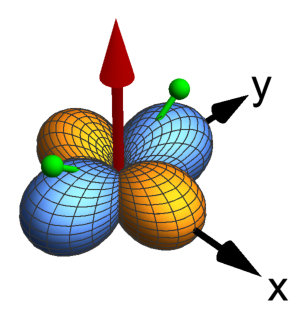
\includegraphics[width=0.25\textwidth]{figures/ch_H2O/1b1_1b2/orbitals.eps}
  \caption{Schematic display of the $1b_{1}\approx 2p_{x}$ (shown in
    yellow along the $x$ axis) and $1b_{2}\approx 2p_{y}$ (shown in
    blue along the $y$ axis) molecular orbitals. Also indicated (in
    green on the $y-z$ plane) is the location of the protons. The $z$
    axis (in red) is the direction of the external electric field of
    strength $F_{0}$.}
  \label{fig:h2o_1b1_1b2}
\end{figure}

As a first step in solving Eq.~(\ref{eq:sch_noCS}) for the H$_{2}$O
molecular orbitals, we introduce the reduced single-centre Moccia
wave function,
%
\begin{eqnarray}
  \begin{split}
    \psi_{1b_{1},1b_{2}}^{nlm}(r) & = & \sum\limits_{i}
    c_{nlm} f_{nlm}(\zeta_{i}, r),
    \label{eq:sto_1b1_1b2}
  \end{split}
\end{eqnarray}
%
which approximates the molecular orbital by an eigenstate of a
spherically symmetric potential. The functions $f_{nlm}(\zeta_{i},r)$
represent the radial part of the Slater orbitals~(\ref{eq:f_STO}) with
$|m|=1$ for the magnetic quantum number, in which the \textsc{sto}
expansion is limited to $2p_{x}$ and $2p_{y}$ orbitals,
respectively. The set of expansion coefficients and non-linear
coefficients in~(\ref{eq:sto_1b1_1b2}), indicated in
Table~\ref{tab:1b11b2_coef}, represents a reduced selection of the
expansion parameters given by Moccia for the ground state of the water
molecule~\cite{Moccia_1964}.

\begin{table}[t]
 \centering
  \caption{\label{tab:1b11b2_coef} Expansion coefficients and
    nonlinear coefficients for the $1b_{1}$ and $1b_{2}$ molecular
    orbitals of H$_{2}$O. The parameters used in our reduced
    \textsc{sto} expansion are indicated as included.}
  \begin{tabular}{lrrrr}
    \toprule
    $(n,l, m)$ & & $\zeta_{i}$ & $c_{nlm}^{1b_{1}}$ & $c_{nlm}^{1b_{2}}$ \\
    \midrule
    $(2,1,1)$ & included & $1.510$ & $0.72081$ & --~~ \\
    $(2,1,1)$ & included & $2.440$ & $0.11532$ & --~~ \\
    $(2,1,1)$ & included & $3.920$ & $0.24859$ & --~~ \\
    $(3,2,1)$ & excluded & $1.600$ & $0.05473$ & --~~ \\
    $(3,2,1)$ & excluded & $2.400$ & $0.00403$ & --~~ \\
    $(4,3,1)$ & excluded & $1.950$ & $0.00935$ & --~~ \\
    $(4,3,3)$ & excluded & $1.950$ & $-0.02691$ & --~~ \\
    $(2,1,-1)$ & included & $1.510$ & --~~ & $0.88270$ \\
    $(2,1,-1)$ & included & $2.440$ & --~~ & $-0.07083$ \\
    $(2,1,-1)$ & included & $3.920$ & --~~ & $0.23189$ \\
    $(3,2,-1)$ & excluded & $1.600$ & --~~ & $0.25445$ \\
    $(3,2,-1)$ & excluded & $2.400$ & --~~ & $-0.01985$ \\
    $(4,3,-1)$ & excluded & $1.950$ & --~~ & $0.04526$ \\
    $(4,3,-3)$ & excluded & $1.950$ & --~~ & $-0.06381$ \\
    \bottomrule
  \end{tabular}
\end{table}

In order to determine the effective potential corresponding to each
molecular orbital, the wave function~(\ref{eq:sto_1b1_1b2}) is inserted
into the single-electron Schr\"{o}dinger equation~(\ref{eq:sch_noCS}),
which is then solved for $V_{\mathrm{eff}}^{(1)}(r)$. Afterwards, the
so-called Latter correction~\cite{LatterCor_1955,sarias_2016} is
applied to ensure that the effective potential converges
asymptotically to $-1/r$, as expected in a Coulomb potential:
%
\begin{eqnarray}
V_{\mathrm{eff}}(r) = \left\{
\begin{split}
V_{\mathrm{eff}}^{(1)}(r)\  & \mathrm{for} & r < r_{0} \\
-1/r\  & \mathrm{for} & r > r_{0}
\end{split}
\right.
,
\label{eq:coulomb_tail}
\end{eqnarray}
%
where the point $r_{0}$ is determined from $V_{\mathrm{eff}}^{(1)}(r_{0}) =
-1/r_{0}$, and is found to be sufficiently large that the original
self-consistent field orbital energy used to derive
$V_{\mathrm{eff}}^{(1)}(r)$ is close to the eigenenergy
of~(\ref{eq:sch_noCS}), with at least two significant digits of
agreement, with $V_{\mathrm{eff}}(r)$ given
by~(\ref{eq:coulomb_tail}).

\begin{figure}
  \centering
  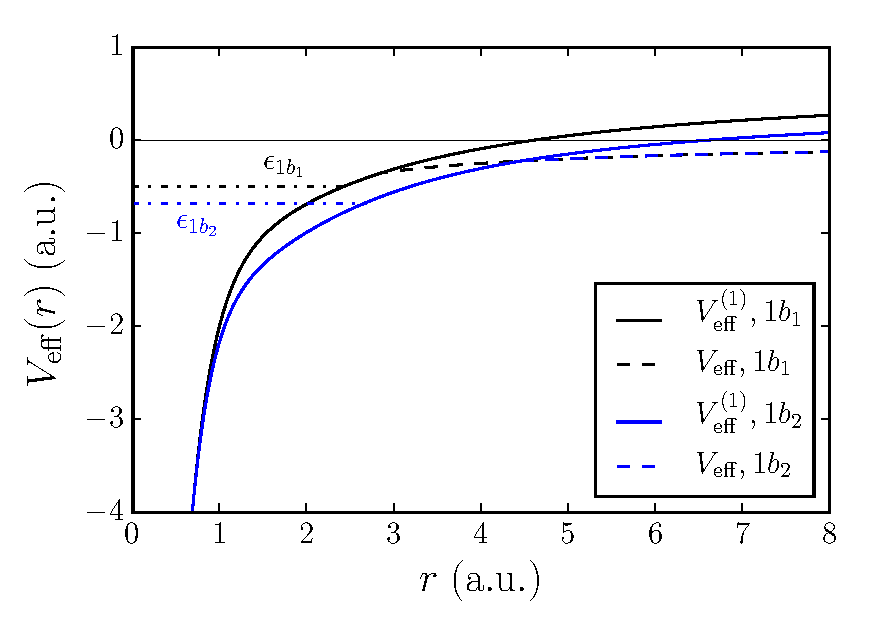
\includegraphics[width=0.75\textwidth]{figures/ch_H2O/1b1_1b2/Veff1b11b2.eps}
  \caption{Electronic effective potential in atomic units for the
    $1b_{1}\approx 2p_{x}$ (black) and $1b_{2}\approx 2p_{y}$ (blue)
    \textsc{mo}s of the H$_{2}$O molecule. The solid lines give the
    potential as derived from~(\ref{eq:sch_noCS}) using the
    \textsc{scf} orbitals and eigenenergies, while the dashed lines
    show the potentials after the Latter correction is applied. The
    dot-dashed lines indicate the eigenenergies obtained from the
    Moccia wave functions~\cite{Moccia_1964}.}
  \label{fig:Veff1b11b2}
\end{figure}

Figure~\ref{fig:Veff1b11b2} shows a comparison of the effective
potential $V_{\mathrm{eff}}^{(1)}(r)$ (solid lines), with black
representing the $1b_{1}$ \textsc{mo} and blue representing the
$1b_{2}$ \textsc{mo}, derived from the Moccia wave functions
representing the $1b_{1}$ and $1b_{2}$
\textsc{mo}s~\cite{Moccia_1964}, and the transformed electronic
potential $V_{\mathrm{eff}}(r)$ (dashed lines) after the Latter
correction was implemented. The effective potentials for the $1b_{1}$
and $1b_{2}$ \textsc{mo}s are given as the shallower and deeper
curves. As Figure~\ref{fig:Veff1b11b2} illustrates, one drawback of
the method is that the effective potential is orbital dependent. A
direct consequence is that the value of $r=r_{0}$, which sets the
position in $r$ where the Coulombic tail is imposed, differs between
the \textsc{mo}s, being almost two times larger for the $1b_{2}$
compared to the $1b_{1}$ \textsc{mo}.


\subsection{PDE approach and exterior complex scaling}
\label{ch:ecs_1b11b2}

This section discusses further the formalism implemented to calculate
the relevant resonance parameters in the problem of the H$_{2}$O
molecule exposed to a strong dc field. Having obtained an effective
potential to define the field-free Schr\"{o}dinger
equation~(\ref{eq:sch_noCS}) for an orbital obtained in the
\textsc{scf} method~\cite{Moccia_1964}, we proceed with the problem of
the molecule ionized by a strong dc field.

When an electric field is applied in the $\hat{z}$ direction,
$\mathbf{F} = F_{0}\hat{z}$, the separation of variables ansatz as
applied to the Schr\"{o}dinger equation~(\ref{eq:sch_noCS})
%
\begin{eqnarray}
  \begin{split}
    \psi(r,\theta,\phi) & = & \psi(r,\theta)\exp(im\phi)
  \end{split}
\label{eq:sov}
\end{eqnarray}
%
leads to a partial differential equation (\textsc{pde}) in spherical
coordinates that represents the Stark problem for an H$_{2}$O orbital:
%
\begin{eqnarray}
 \begin{split}
  -\frac{1}{2} \frac{\partial^{2}\psi}{\partial r^2} - \frac{1}{2r^2}
  (\frac{\cos\theta}{\sin\theta} \frac{\partial\psi}{\partial\theta} + 
  \frac{\partial^2\psi}{\partial\theta^2})
  + (\frac{m^2}{2r^2 \sin^2\theta} + V_{\mathrm{eff}}(r) - E +
  F_{0}r\cos\theta)\psi & = & 0.
  \end{split}
\label{eq:pde}
\end{eqnarray}
%
Here the complex eigenenergy $E$ contains the information about the
resonance position (real part), i.e., $E_{R}$ and width $\Gamma$
(imaginary part is $-\Gamma/2$), and may be expressed as
%
\begin{eqnarray}
E & = & E_{R} + iE_{I} = E_{R} - i\frac{\Gamma}{2}.
\label{eq:complex_E}
\end{eqnarray}
%
% EXPLAIN HERE THAT M=\PM-1 ARE THE 2P_1 AND 2P_-1 EIGENSTATES OF L_Z
% AND 2P_X AND 2P_Y ARE LINEAR COMBINATIONS OF THESE L_Z EIGENSTATES
The imaginary part $\Gamma$ is related to the lifetime of the decaying
state $\tau$ via $\Gamma\tau = 1$. For the $1b_{1}$ and $1b_{2}$
orbitals, which are formulated as linear combinations of the $L_{z}$
eigenstates $2p_{x}$ and $2p_{y}$, respectively, we have $|m| = 1$ in
Eq.~(\ref{eq:pde}). The presence of the effective potential
$V_{\mathrm{eff}}(r)$ makes this problem challenging in the sense that
it is not possible to obtain separable solutions like for the hydrogen
atom in which a pure Coulomb potential leads to separability in
parabolic coordinates, as was discussed in~\cite{Telnov_1989}. It is
then necessary to generate a more general solution by solving the
\textsc{pde} numerically, e.g., by applying a finite-element method.

The ionization regime of the water molecule is described by means of a
non-Hermitian Hamiltonian that reveals discrete resonance eigenvalues
containing information about the quasibound states that tunnel through
the barrier or escape over the potential barrier for strong
fields. Among the different techniques implemented in the study of
atomic resonances, a standard tool is the method of complex
scaling~\cite{complexScaling,complexScalingBaslev,complexScalingSimon}. This
approach consists in extending the analytic domain of the Hamiltonian
of a given system by means of a mapping operator that results in
complex eigenvalues which provide direct access to the resonant states
of the Stark problem. For most phenomenological potentials, such as
molecules with fixed internuclear distances, a modified method of
scaling is required as an extension to cases where the potential is
analytic only outside some bounded region. In these cases, the
approach of exterior complex scaling (\textsc{ecs})~\cite{Simon_1979}
is more appropriate, as the potential needs to have analyticity
properties only in the region affected by the scaling, where one can
look for solutions which decay exponentially in the assymptotic region
of the potential. Both methods have been widely used in scattering
problems~\cite{complexScalingBaslev, complexScalingSimon}, in studies
of the Stark problem for multi-electron
systems~\cite{ScrinziJChemPhys_ECS,ScrinziJPhysB_ECS}, as well as in
time-dependent Schr\"{o}dinger equation problems for strong
fields~\cite{ecsRuiz, ecsTao, ecsScrinzi}.

For our aim of studying the field ionization properties of H$_{2}$O
orbitals, we implement a modified \textsc{ecs} technique in which the
radial coordinates are extended into the complex plane by a phase
factor, which is turned on gradually beyond some distance from the
origin. This method allows us to address the tunneling and
over-barrier ionization problem by avoiding the complication of
describing quasibound states with outgoing waves for $r \to
\infty$. In the present work, the complex scaling transformation is
given by
%
\begin{eqnarray}
  \begin{split}
    r & \rightarrow & r\exp(i\chi(r)),
  \end{split}
\label{eq:ecs_r}
\end{eqnarray}
%
where $\chi$ is defined as a function of the $r$ coordinate with the
purpose of making the scaling gradually effective from some vicinity
of $r = r_{\mathrm{s}}$ on,
%
\begin{eqnarray}
  \begin{split}
    \chi(r) & = & \frac{\chi_{\mathrm{s}}}{1+\exp[-\frac{1}{\Delta r}
        (r - r_{\mathrm{s}})]}.
  \end{split}
\label{eq:ecs_theta}
\end{eqnarray} 
%
For given $r_{\mathrm{s}}$ one has to choose $\Delta r$ to be
sufficiently small, so that the function $\chi(r)$ starts from small
values at $r = 0$. For large $r$, it converges to the value
$\chi_{\mathrm{s}}$. Figure~\ref{fig:scaling} illustrates the scaling
function $\chi(r)$ that corresponds to the set of $(\chi_{\mathrm{s}},
r_{\mathrm{s}}, \Delta r)$ values used in the numerical calculations
of the dc Stark parameteres for the H$_{2}$O valence orbitals.

% plot of \chi(r)
\begin{figure}
  \centering
  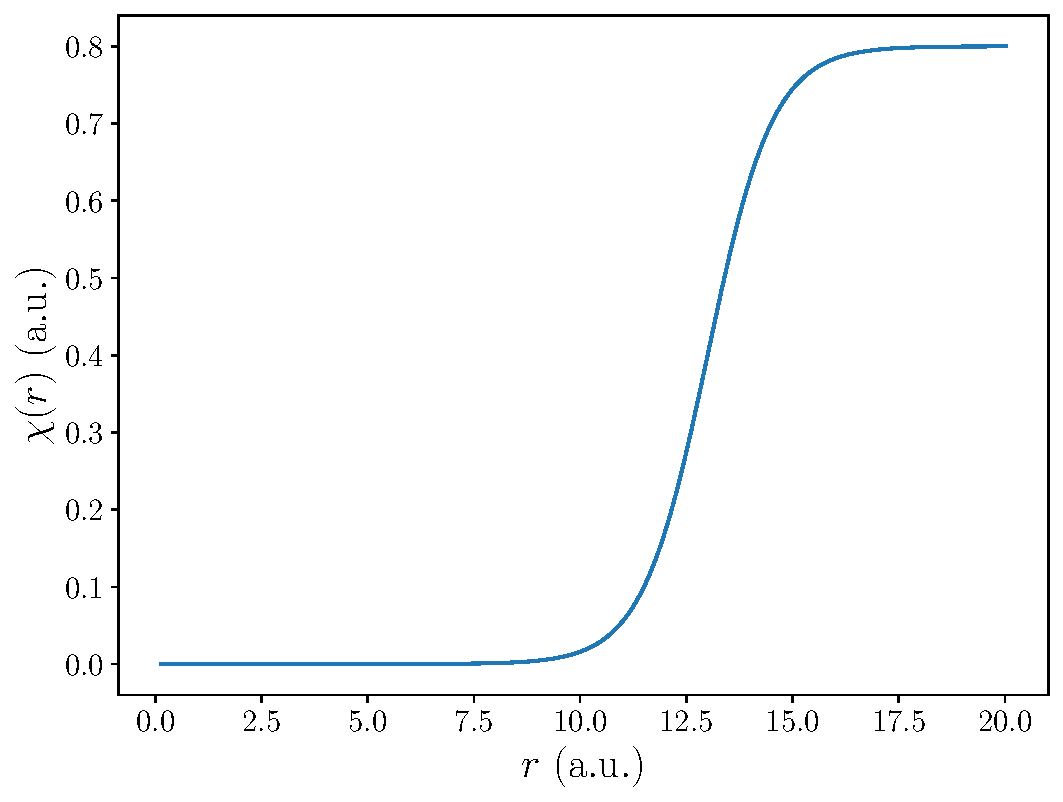
\includegraphics[width=0.6\textwidth]{figures/ch_H2O/1b1_1b2/scaling.pdf}
  \caption{Scaling function corresponding to $\chi_{\mathrm{s}} =
    0.8\ \mathrm{a.u.}$, $r_{\mathrm{s}} = 13\ \mathrm{a.u.}$, and $1
    / \Delta r = 1.3\ \mathrm{a.u.}$}
  \label{fig:scaling}
\end{figure}


The set of possible values for the asymptotic scaling angle
$\chi_{\mathrm{s}}$ and the parameters $r_{\mathrm{s}}$ and $\Delta
r$, which control where and how quickly the scaling is turned on, is
explored in detail in order to establish how sensitive the
\textsc{pde} solutions are and to test the effectiveness of the
complex scaling technique to absorb the outgoing wave. Numerous tests
were carried out to ensure that the ``exact'' results of
Telnov~\cite{Telnov_1989} for atomic hydrogen orbitals including $2p$
are reproduced.

In order to investigate the effects of the dc field on the H$_{2}$O
orbital energies it is necessary to consider the extra terms that the
\textsc{ecs}~(\ref{eq:ecs_r}) introduces in the Schr\"{o}dinger
equation~(\ref{eq:pde}). Additionally, we need to turn the scaling on
only in the regime $r > r_{0}$, as Eq.~(\ref{eq:coulomb_tail})
indicates, such that we have a simple Coulomb potential in the scaling
region. In order to make use of standard finite-element methods, the
complex-valued wave function is separated into real and imaginary
parts, such that a system of coupled differential equations is
obtained as follows~\cite{sarias_2016}:
%
\begin{eqnarray}
  -\frac{1}{2}\frac{\partial^{2}\psi_{R}}{\partial r^2}-\frac{1}{2r^2}
  (\frac{\cos\theta}{\sin\theta}\frac{\partial\psi_{R}}{\partial\theta}+
  \frac{\partial^{2}\psi_{R}}{\partial\theta^2}) \nonumber\\
  +(\frac{m^2}{2r^2\sin^2\theta}+V_{\rm{eff}}^{R}(r)c_{2}-V_{\rm{eff}}^{I}(r)s_{2}
  -E_{R}c_{2}+E_{I}s_{2}+
  F_{0}r\cos\theta c_{3})\psi_{R} \nonumber\\
  +(-V_{\rm{eff}}^{R}(r)s_{2}-V_{\rm{eff}}^{I}(r)c_{2}+E_{R}s_{2}+E_{I}c_{2}-F_{0}r\cos\theta
  s_{3})\psi_{I} & = & 0, \nonumber\\
  \vspace{1cm}
  -\frac{1}{2}\frac{\partial^{2}\psi_{I}}{\partial r^2}-\frac{1}{2r^2}
  (\frac{\cos\theta}{\sin\theta}\frac{\partial\psi_{I}}{\partial\theta}+
  \frac{\partial^{2}\psi_{I}}{\partial\theta^2}) \nonumber\\
  +(\frac{m^2}{2r^2\sin^2\theta}+V_{\rm{eff}}^{R}(r)c_{2}-V_{\rm{eff}}^{I}(r)s_{2}
  -E_{R}c_{2}+E_{I}s_{2}+
  F_{0}r\cos\theta c_{3})\psi_{I} \nonumber\\
  +(V_{\rm{eff}}^{R}(r)s_{2}+V_{\rm{eff}}^{I}(r)c_{2}-E_{R}s_{2}-E_{I}c_{2}+F_{0}r\cos\theta
  s_{3})\psi_{R} & = & 0.
\label{eq:pde_system}
\end{eqnarray}
%
The labels $R$ and $I$ stand for real and imaginary parts,
respectively; also, the notation $[c_{k},s_{k}]$ is introduced to
represent $[\cos[k\chi(r)], \sin[k\chi(r)]]$, respectively, with
$k=2,3$ and $\chi(r)$ defined in~(\ref{eq:ecs_theta}). Note that the
effective potential has real and imaginary parts on account of the
coordinate transformation~(\ref{eq:ecs_r}).
 
The \textsc{pde} system~(\ref{eq:pde_system}) is solved numerically on
a rectangular mesh defined by the $(r, \theta)$ coordinates, which
take values in the domains $\epsilon < r < r_{\mathrm{max}}$ and $\eta
< \theta < \pi - \eta$, respectively. The parameters $\epsilon$ and
$\eta$, that limit the coordinate ranges to avoid singularities at the
origin, were chosen to be of the order of $10^{-3}\ \mathrm{a.u.}$,
and the $r$ coordinate extends to $r_{\mathrm{max}} =
20\ \mathrm{a.u.}$ In order to find a correct set of
$\psi_{R(I)}(r,\theta)$ solutions, it is essential to impose proper
boundary conditions that ensure the wave functions vanish at the
limits of the mesh. For the $|m| = 1$ states we impose the condition
$\psi_{R{I}}(\epsilon,\theta) = \epsilon \sin(\theta) = \epsilon
P_{1}^{1}(\theta)$, which is consistent with the assumption that at
small $r = \epsilon$ the lowest term in an expansion in associated
Legendre polynomials dominates and behaves like $A r^{2}
\sin(\theta)$.

A two-parameter root search for $\{E_{R}, E_{I}\}$ is implemented by
solving the \textsc{pde} as if it were an inhomogeneous problem. We
pick a location in the $(r,\theta)$ plane where the probability
amplitude is expected to be large and vary $\{E_{R}, E_{I}\}$, i.e.,
effectively the complex energy $E$ to maximize the amplitude.


\section{$3a_{1}$ molecular orbital}
\label{ch:3a1}

% sec 2 of JPhysB
In this section we extend the approach to study the dc Stark problem
for the $3a_{1}$ molecular orbital of H$_{2}$O. Given the orientation
of this orbital with respect to the plane in which the two protons are
located it is deemed necessary to go beyond the spherical effective
potential approximation, which was implemented in
Sec.~\ref{ch:1b1_1b2} for the $1b_{1}$ and $1b_{2}$ orbitals, in order
to take into account the strong asymmetry introduced by the protons in
the $y-z$ plane and the significant admixtures of $s-$type Slater
orbitals in the \textsc{sto}s~\cite{Moccia_1964}.

The proposed method to address this problem is to define a reduced
single-centre Moccia wave function,
%
\begin{eqnarray}
\psi_{3a_{1}}(r,\theta) = \sum_{n,l} c_{nl0} \varphi_{nl}(r,\theta).
\label{eq:3a1Moccia_expansion}
\end{eqnarray}
%
Here the $\varphi_{nl}(r,\theta)$ are Slater orbitals with $m=0$ for
the magnetic quantum number, and we limited the expansion to
\textsc{sto}s of $2s$ and $2p_{z}$ type. The parameters are given in
Table~\ref{tab:3a1_coef} and three $2p_{z}$ orbitals are mixed with
three $2s$-type orbitals. This set of coefficients represents a
reduced selection of the expansion parameters given by Moccia for the
ground state of the water molecule~\cite{Moccia_1964} also shown in
Table~\ref{tab:3a1_coef}.

\begin{table}[t]
\centering
\caption{\label{tab:3a1_coef} Expansion coefficients and non-linear
  coefficients for the $3a_{1}$ \textsc{mo}. The parameters used in
  our reduced \textsc{sto} expansion are indicated as included.}
\begin{tabular}{lrrr}
\toprule
$(n,l,m)$ & & $c_{nlm}$ & $\zeta_{i}$ \\
\midrule[0.25pt]
 $(1,0,0)$ & excluded & $-0.00848$ & $12.600$ \\
 $(1,0,0)$ & excluded & $0.08241$ & $7.450$ \\
\midrule[0.25pt]
 $(2,1,0)$ & included & $0.79979$ & $1.510$  \\
 $(2,1,0)$ & included & $0.00483$ & $2.440$  \\
 $(2,1,0)$ & included & $0.24413$ & $3.920$  \\
 $(2,0,0)$ & included & $-0.30752$ & $2.200$ \\
 $(2,0,0)$ & included & $-0.04132$ & $3.240$ \\
 $(2,0,0)$ & included & $0.14954$ & $1.280$ \\
\midrule[0.25pt]
 $(3,2,0)$ & excluded & $0.05935$ & $1.600$ \\
 $(3,2,0)$ & excluded & $0.00396$ & $2.400$ \\
 $(3,2,2)$ & excluded & $-0.09293$ & $1.600$ \\
 $(3,2,2)$ & excluded & $0.01706$ & $2.400$ \\
 $(4,3,0)$ & excluded & $-0.01929$ & $1.950$ \\
 $(4,3,2)$ & excluded & $-0.06593$ & $1.950$ \\
\bottomrule
\end{tabular}
\end{table}

The probability densities for the $3a_{1}$ orbital as obtained from
the reduced expansion~(\ref{eq:3a1Moccia_expansion}) and from the
Moccia self-consistent results are shown in
Figures~\ref{fig:3a1_reduced} and~\ref{fig:3a1_Moccia},
respectively. The protons (in red) lie in the $y-z$ plane. As
Fig.~\ref{fig:3a1_reduced} indicates, the contributions to the density
of the $2s-$type states reproduce the proper dependence of the
$3a_{1}$ probability density with the polar angle $\theta$, as the
broader hump is located on the negative $z-$axis in the same way as in
the complete Moccia representation shown in Fig.~\ref{fig:3a1_Moccia}.

\begin{figure}
  \centering
  \begin{subfigure}[b]{0.25\linewidth}
    \centering
    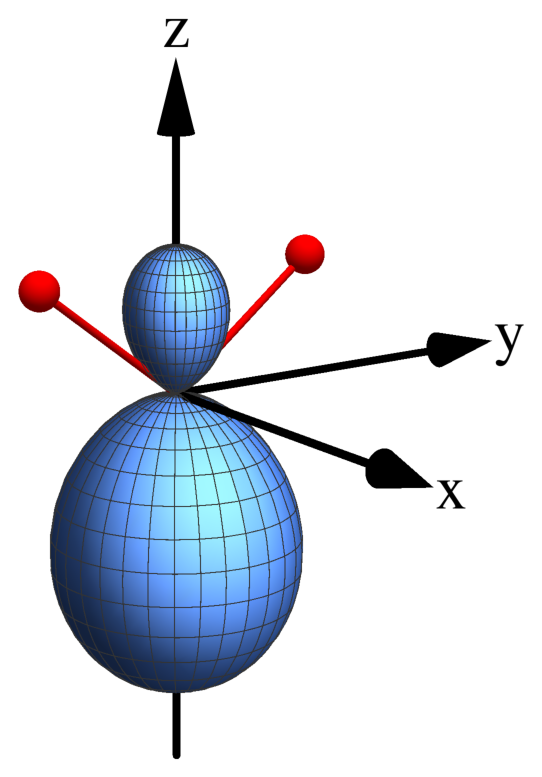
\includegraphics[width=\textwidth]{figures/ch_H2O/3a1/3a1extended.eps}
    \caption{Simplified $3a_{1}$ orbital}\label{fig:3a1_reduced}
  \end{subfigure}
  \,
  \begin{subfigure}[b]{0.25\linewidth}
    \centering
    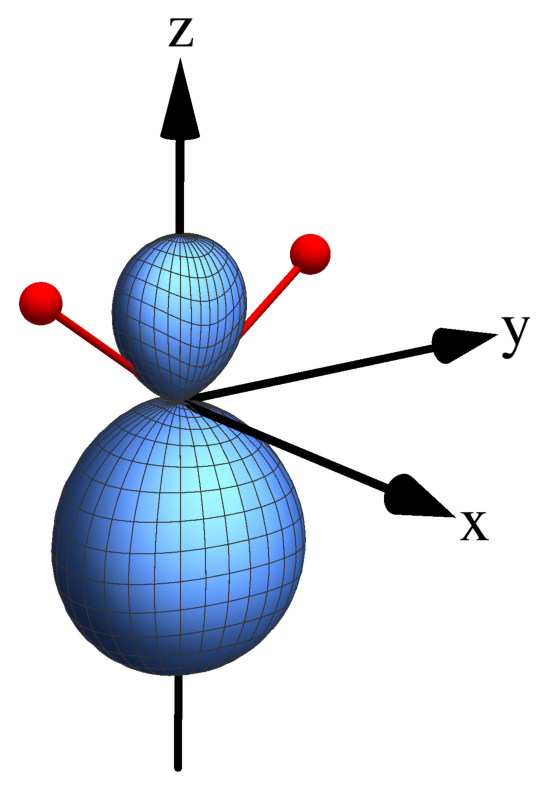
\includegraphics[width=\textwidth]{figures/ch_H2O/3a1/3a1Moccia.eps}
    \caption{Full Moccia $3a_{1}$ orbital}\label{fig:3a1_Moccia}
  \end{subfigure}
  \caption{Schematic display of the $3a_{1}$ molecular orbital (shown
    in blue along the $z$ axis) used to construct
    $V_{\mathrm{eff}}(r,\theta)$. The orbital obtained from a reduced
    expansion in \textsc{sto}s is shown in~(\ref{fig:3a1_reduced}),
    and the complete Moccia orbital is shown
    in~(\ref{fig:3a1_Moccia}). Also indicated (in red in the $y-z$
    plane) is the location of the protons. The $\hat{z}-$axis is the
    direction along which the external electric field of strength
    $F_{0}$ is applied.}
  \label{fig:3a1_prob_density}
\end{figure}

In order to illustrate the fraction of the full Moccia expansion that
our reduced wave function~(\ref{eq:3a1Moccia_expansion}) represents,
the projections of the probability densities over the $x-y$ plane are
shown as contours of constant density in
Figure~\ref{fig:3a1_xycontours}, for the height where the protons are
located. From the complete Moccia representation of the $3a_{1}$
\textsc{mo} (in dashed lines), one observes that the location of the
protons (shown as red circles) has an influence on the shape of the
upper lobe in the probability density, i.e., it introduces dependence
on the azimuthal angle $\varphi$. In our simplified expansion, where
only $l=0,1$ and $m=0$ symmetrical parts were included (shown with
solid lines), the probability density misses to represent the proper
azimuthal dependence that follows from the $m\neq 0$ parts.

\begin{figure}
  \centering
  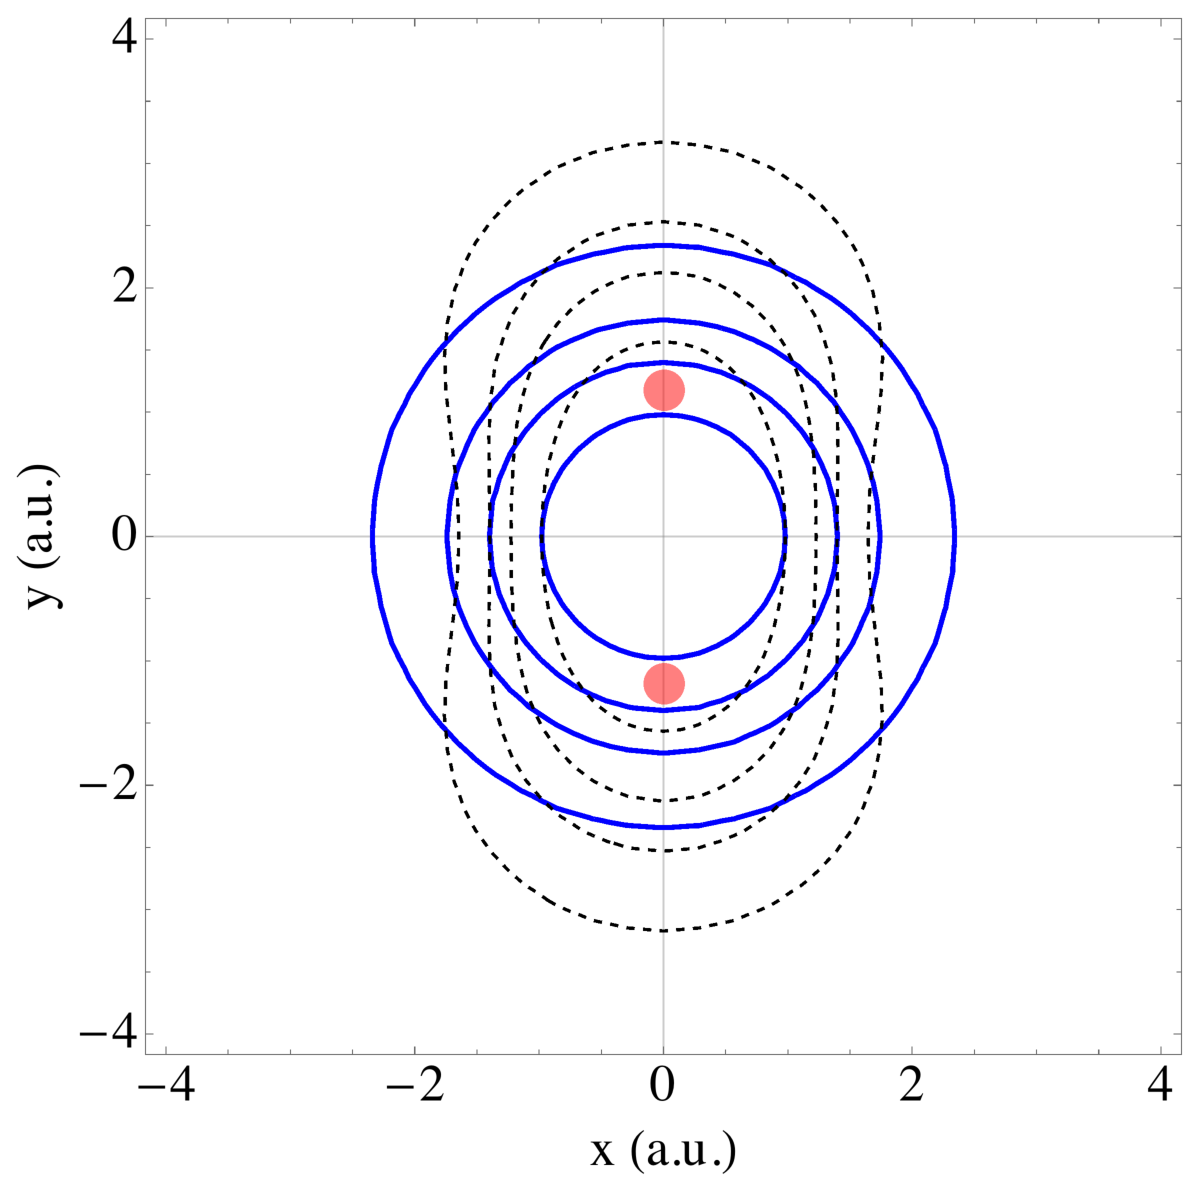
\includegraphics[width=0.6\textwidth]{figures/ch_H2O/3a1/orbitals3a1.eps}
  \caption{Projections of the probability densities for the $3a_{1}$
    orbital on the $x-y$ plane. The simplified \textsc{sto} expansion
    is shown by continuous blue lines, and the full Moccia expansion
    is represented by black dashed lines. The proton locations are
    indicated as red circles. The chosen contour values are $0.5, 0.3,
    0.2, 0.1$ starting from the innermost contour.}
  \label{fig:3a1_xycontours}
\end{figure}

The non-spherical effective potential corresponding to the
\textsc{sto} expansion~(\ref{eq:3a1Moccia_expansion}),
$V_{\mathrm{eff}}(r,\theta)$, is obtained from the Schr\"{o}dinger
equation in spherical polar coordinates,
%
\begin{eqnarray}
  \left[ -\frac{1}{2} \nabla^{2} +
  V_{\rm{eff}}(r,\theta) \right] \psi_{3a_{1}}(r,\theta) =
  E_{3a_{1}} \psi_{3a_{1}}(r,\theta).
\label{eq:sch_eq3d}
\end{eqnarray}
%
For given $E_{3a_{1}}$ and $\psi_{3a_{1}}(r,\theta)$ it is
straightforward to solve~(\ref{eq:sch_eq3d}) for
$V_{\mathrm{eff}}(r,\theta)$. In order to use this potential to define
a Hamiltonian for the $3a_{1}$ orbital in an electric field, an
asymptotic Latter correction needs to be applied.

Other strategies for finding an effective potential could be pursued,
such as using a density functional, inserting the Moccia wave function,
and then performing an azimuthal angle average. Ultimately, one would
like to extend density functional theory~(\textsc{dft}) from finding
ground-state energies to obtaining resonance positions and
widths. This might be feasible using a combination of time-dependent
\textsc{dft} and Floquet theory. The goal of the present work is more
modest: we calculate the response of an isolated molecular orbital in
a simple approximation. Recently, the problem of small molecules in a
dc field has revealed the effect of electron-electron interactions on
Stark resonance parameters~\cite{ScrinziJPhysB_ECS}. It will be
interesting to observe such effects for the water molecule in future
work.


\subsection{Interpolation and Latter correction of the
  non-spherical effective potential}
\label{ch:3a1_Latter}

The non-central effective potential, $V_{\mathrm{eff}}(r,\theta)$,
leads no longer to an orbital of $(l,m)$ symmetry for the case of the
$3a_{1}$ orbital. This reflects the geometry of the problem as a
consequence of the location of the protons. The use of this more
general potential implies that the Latter
criterion~\cite{LatterCor_1955}, which ensures the proper asymptotic
behaviour of the potential, is not as straightforward to implement as
in the case of the spherical potential discussed in
Sec.~\ref{ch:1b1_1b2}, where the correction applies beyond a
determined $r$ value~\cite{sarias_2016}. In this case, the correction
must be implemented in the $r-\theta$ plane, by defining a
$\theta-$dependent boundary beyond which the potential obtained
from~(\ref{eq:sch_eq3d}) rises above $-1/r$ in the asymptotic
region~\cite{sarias_2017}.

The $\theta$ coordinate is fixed at two extreme positions, such as
$\theta = 0$ and $\theta = \pi$, in order to find the corresponding
$r$ values $r_{0}$ and $r_{\pi}$, for which
$V_{\mathrm{eff}}(r,\theta) = -1/r$ is satisfied, then we interpolate
between them by introducing the $\theta-$dependent function
%
\begin{eqnarray}
r_{\rm{match}}(\theta) & = & \bar{r} - (r_{\pi} - \bar{r}) \cos\theta,
\label{eq:rMatch}
\end{eqnarray}
%
where $\bar{r} = (r_{0} + r_{\pi})/2$. With this approach we redefine
the effective potential to be the non-central potential derived from
the reduced Moccia wave function using Equation~(\ref{eq:sch_eq3d})
when $r < r_{\mathrm{match}}(\theta)$, and $-1/r$ otherwise.

The weighted functions used to construct the Moccia
orbitals~\cite{Moccia_1964} imply a potential difficulty in our
problem. Since these functions are not exact solutions of the
Schr\"{o}dinger equation but were obtained from the variational
principle by implementing a self-consistent
calculation~\cite{Moccia_JCP_2164}, there may be regions in the
$(r,\theta)$ domain where $\psi_{3a_{1}}(r,\theta)$ vanishes, whereas
its second derivative remains finite; this produces a nodal line in
the electronic potential. Thus, finding a potential for which our
approximate wave function satisfies a Schr\"{o}dinger equation
represents an intricate problem.

It turns out that the nodal region is so narrow that when solving the
Schr\"{o}dinger equation the kinetic energy term dominates and it is
possible to obtain a solution that remains close to that obtained by
the \textsc{hf} method~\cite{Moccia_1964}, regardless of the fact that
there is a region where the effective potential might diverge.

The probability density exhibits two humps indicating the positions of
the protons, which is consistent with
Figure~\ref{fig:3a1_prob_density}, and the effects of the mixing with
the $s-$state. One may argue that one of the reasons this nodal region
in the potential does not have a negative impact on the results is due
to the way the $3a_{1}$ orbital responds to the effective potential by
avoiding this region, its probability density being distributed as
shown in Figure~\ref{fig:density_contours}. A numerical interpolation
of $V_{\mathrm{eff}}(r,\theta)$ is implemented in order to ensure it
continues smoothly over this problematic region.

\begin{figure}
  \centering
  \begin{subfigure}[b]{0.245\linewidth}
    \centering
    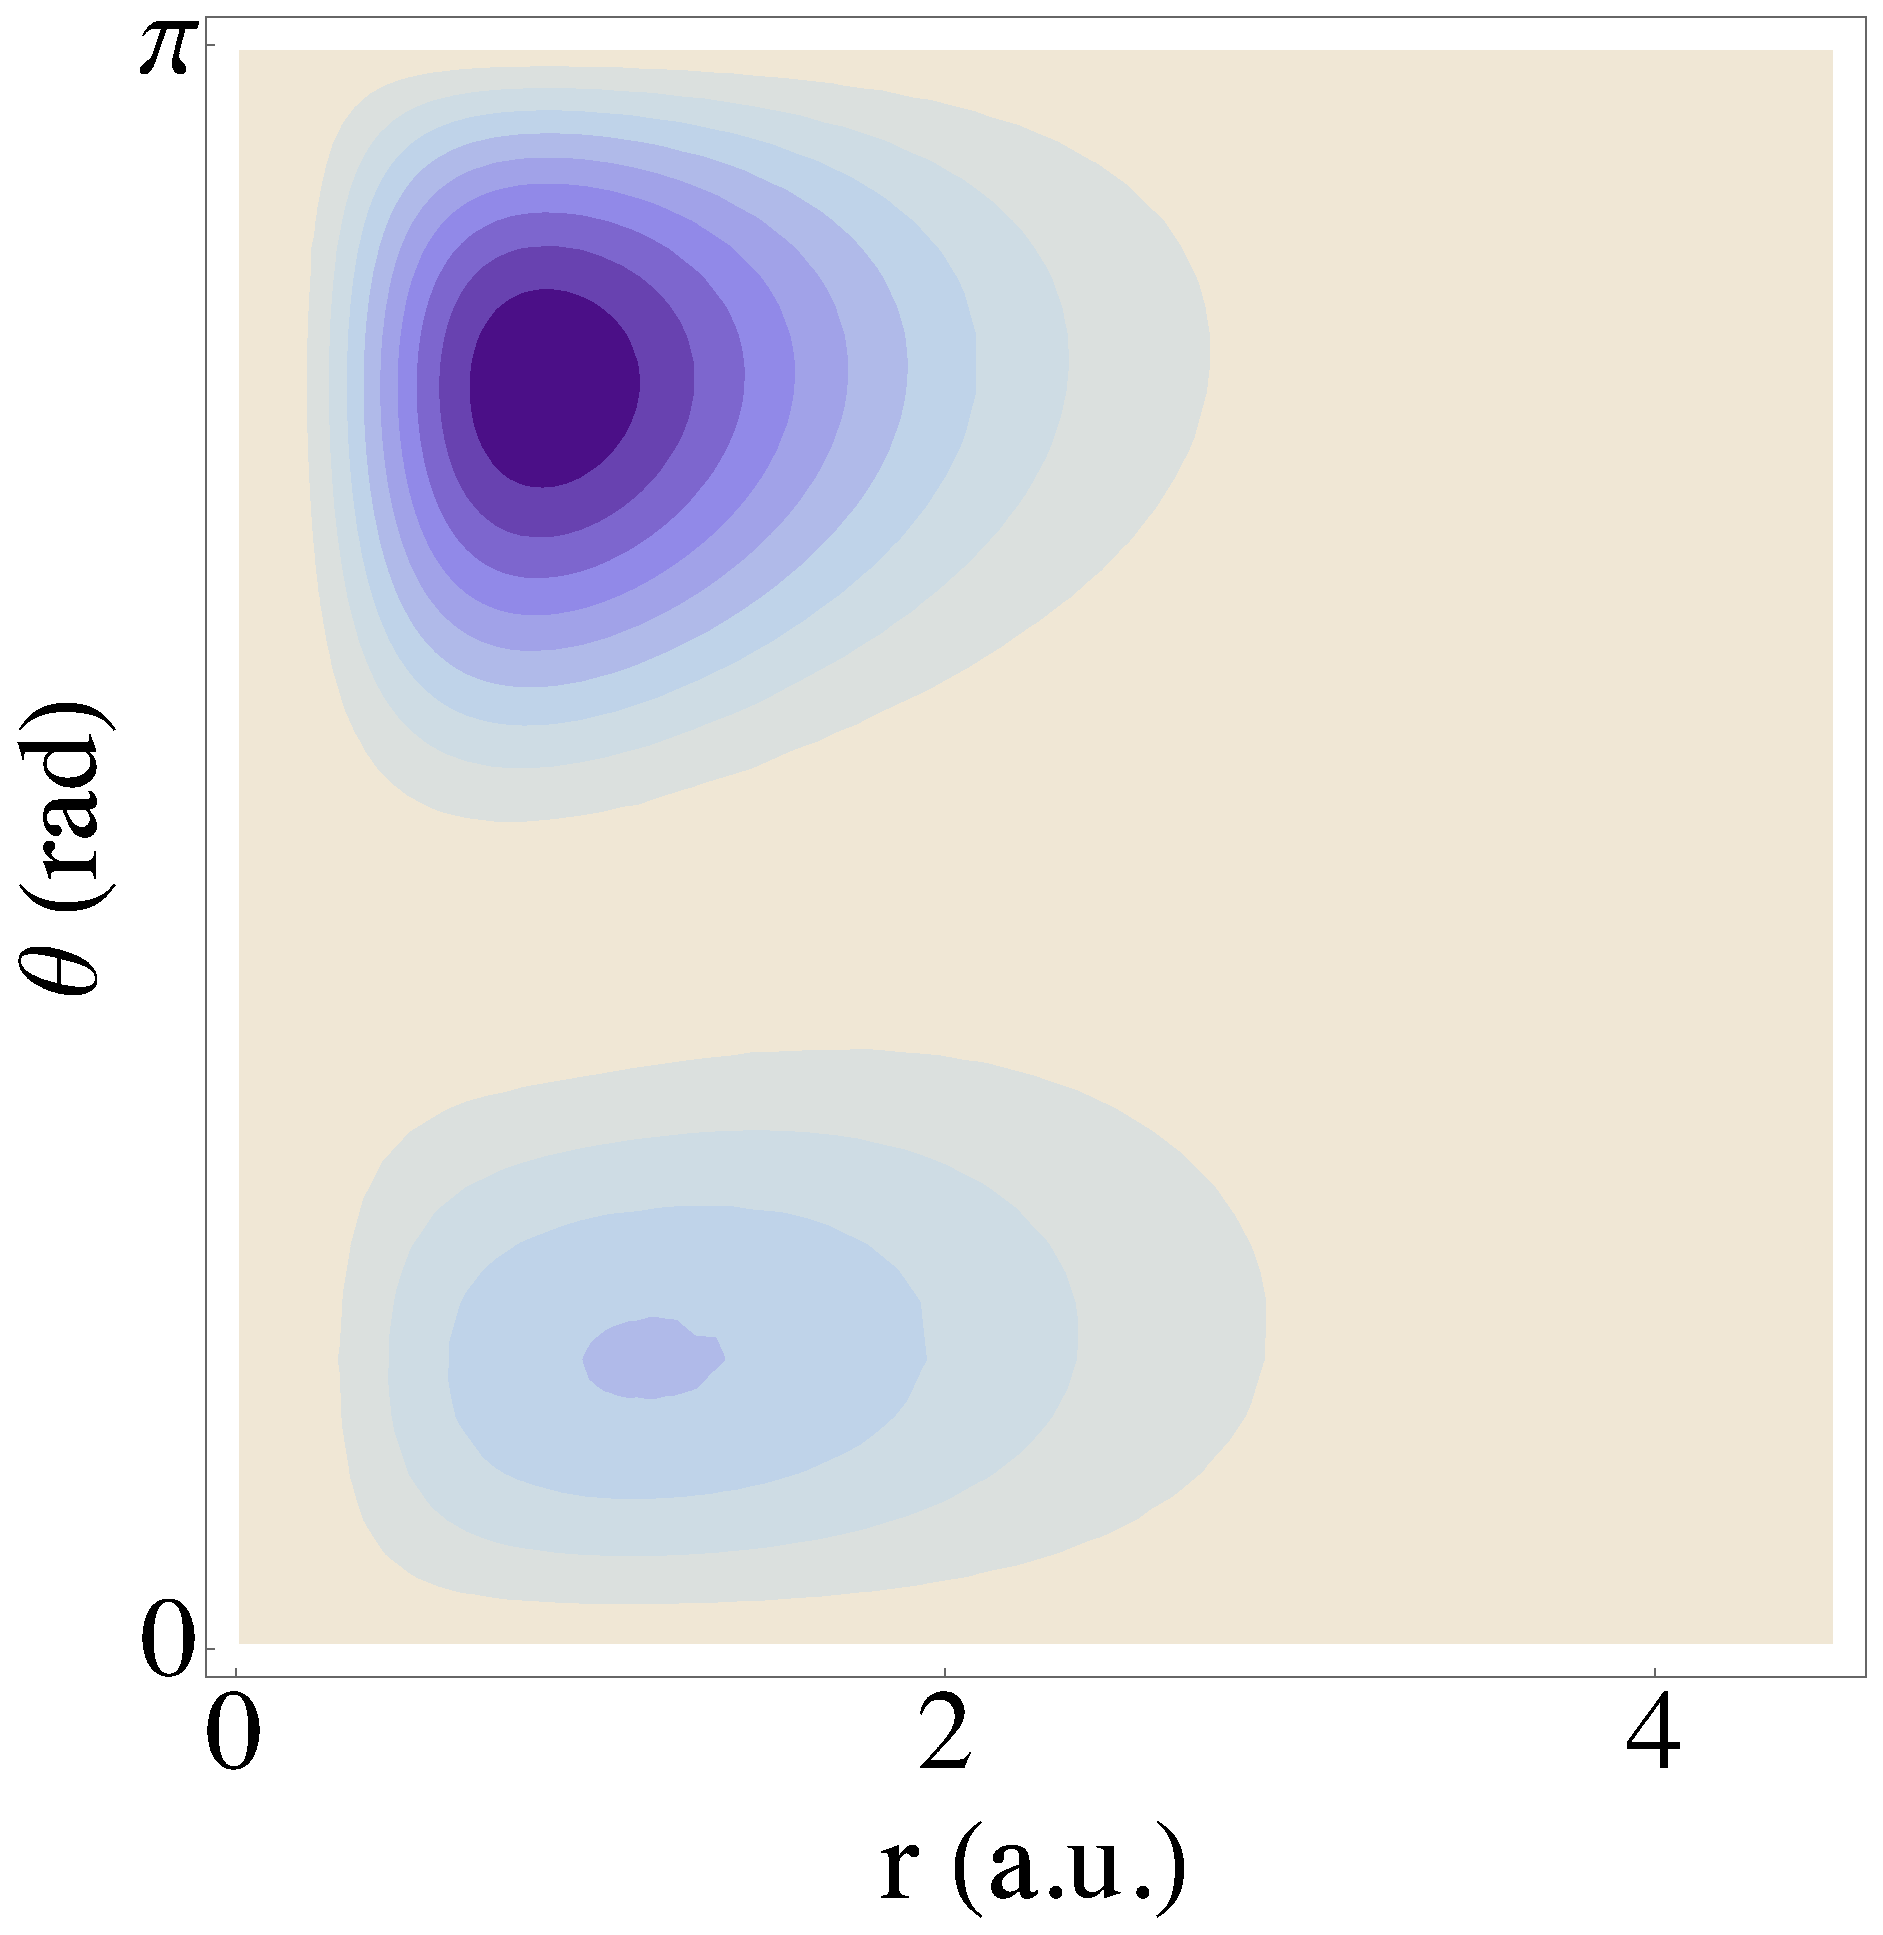
\includegraphics[width=\textwidth]{figures/ch_H2O/3a1/contour3a132s.eps}
    \caption{}\label{fig:Moccia32s}
  \end{subfigure}
  \,
  \begin{subfigure}[b]{0.275\linewidth}
    \centering
    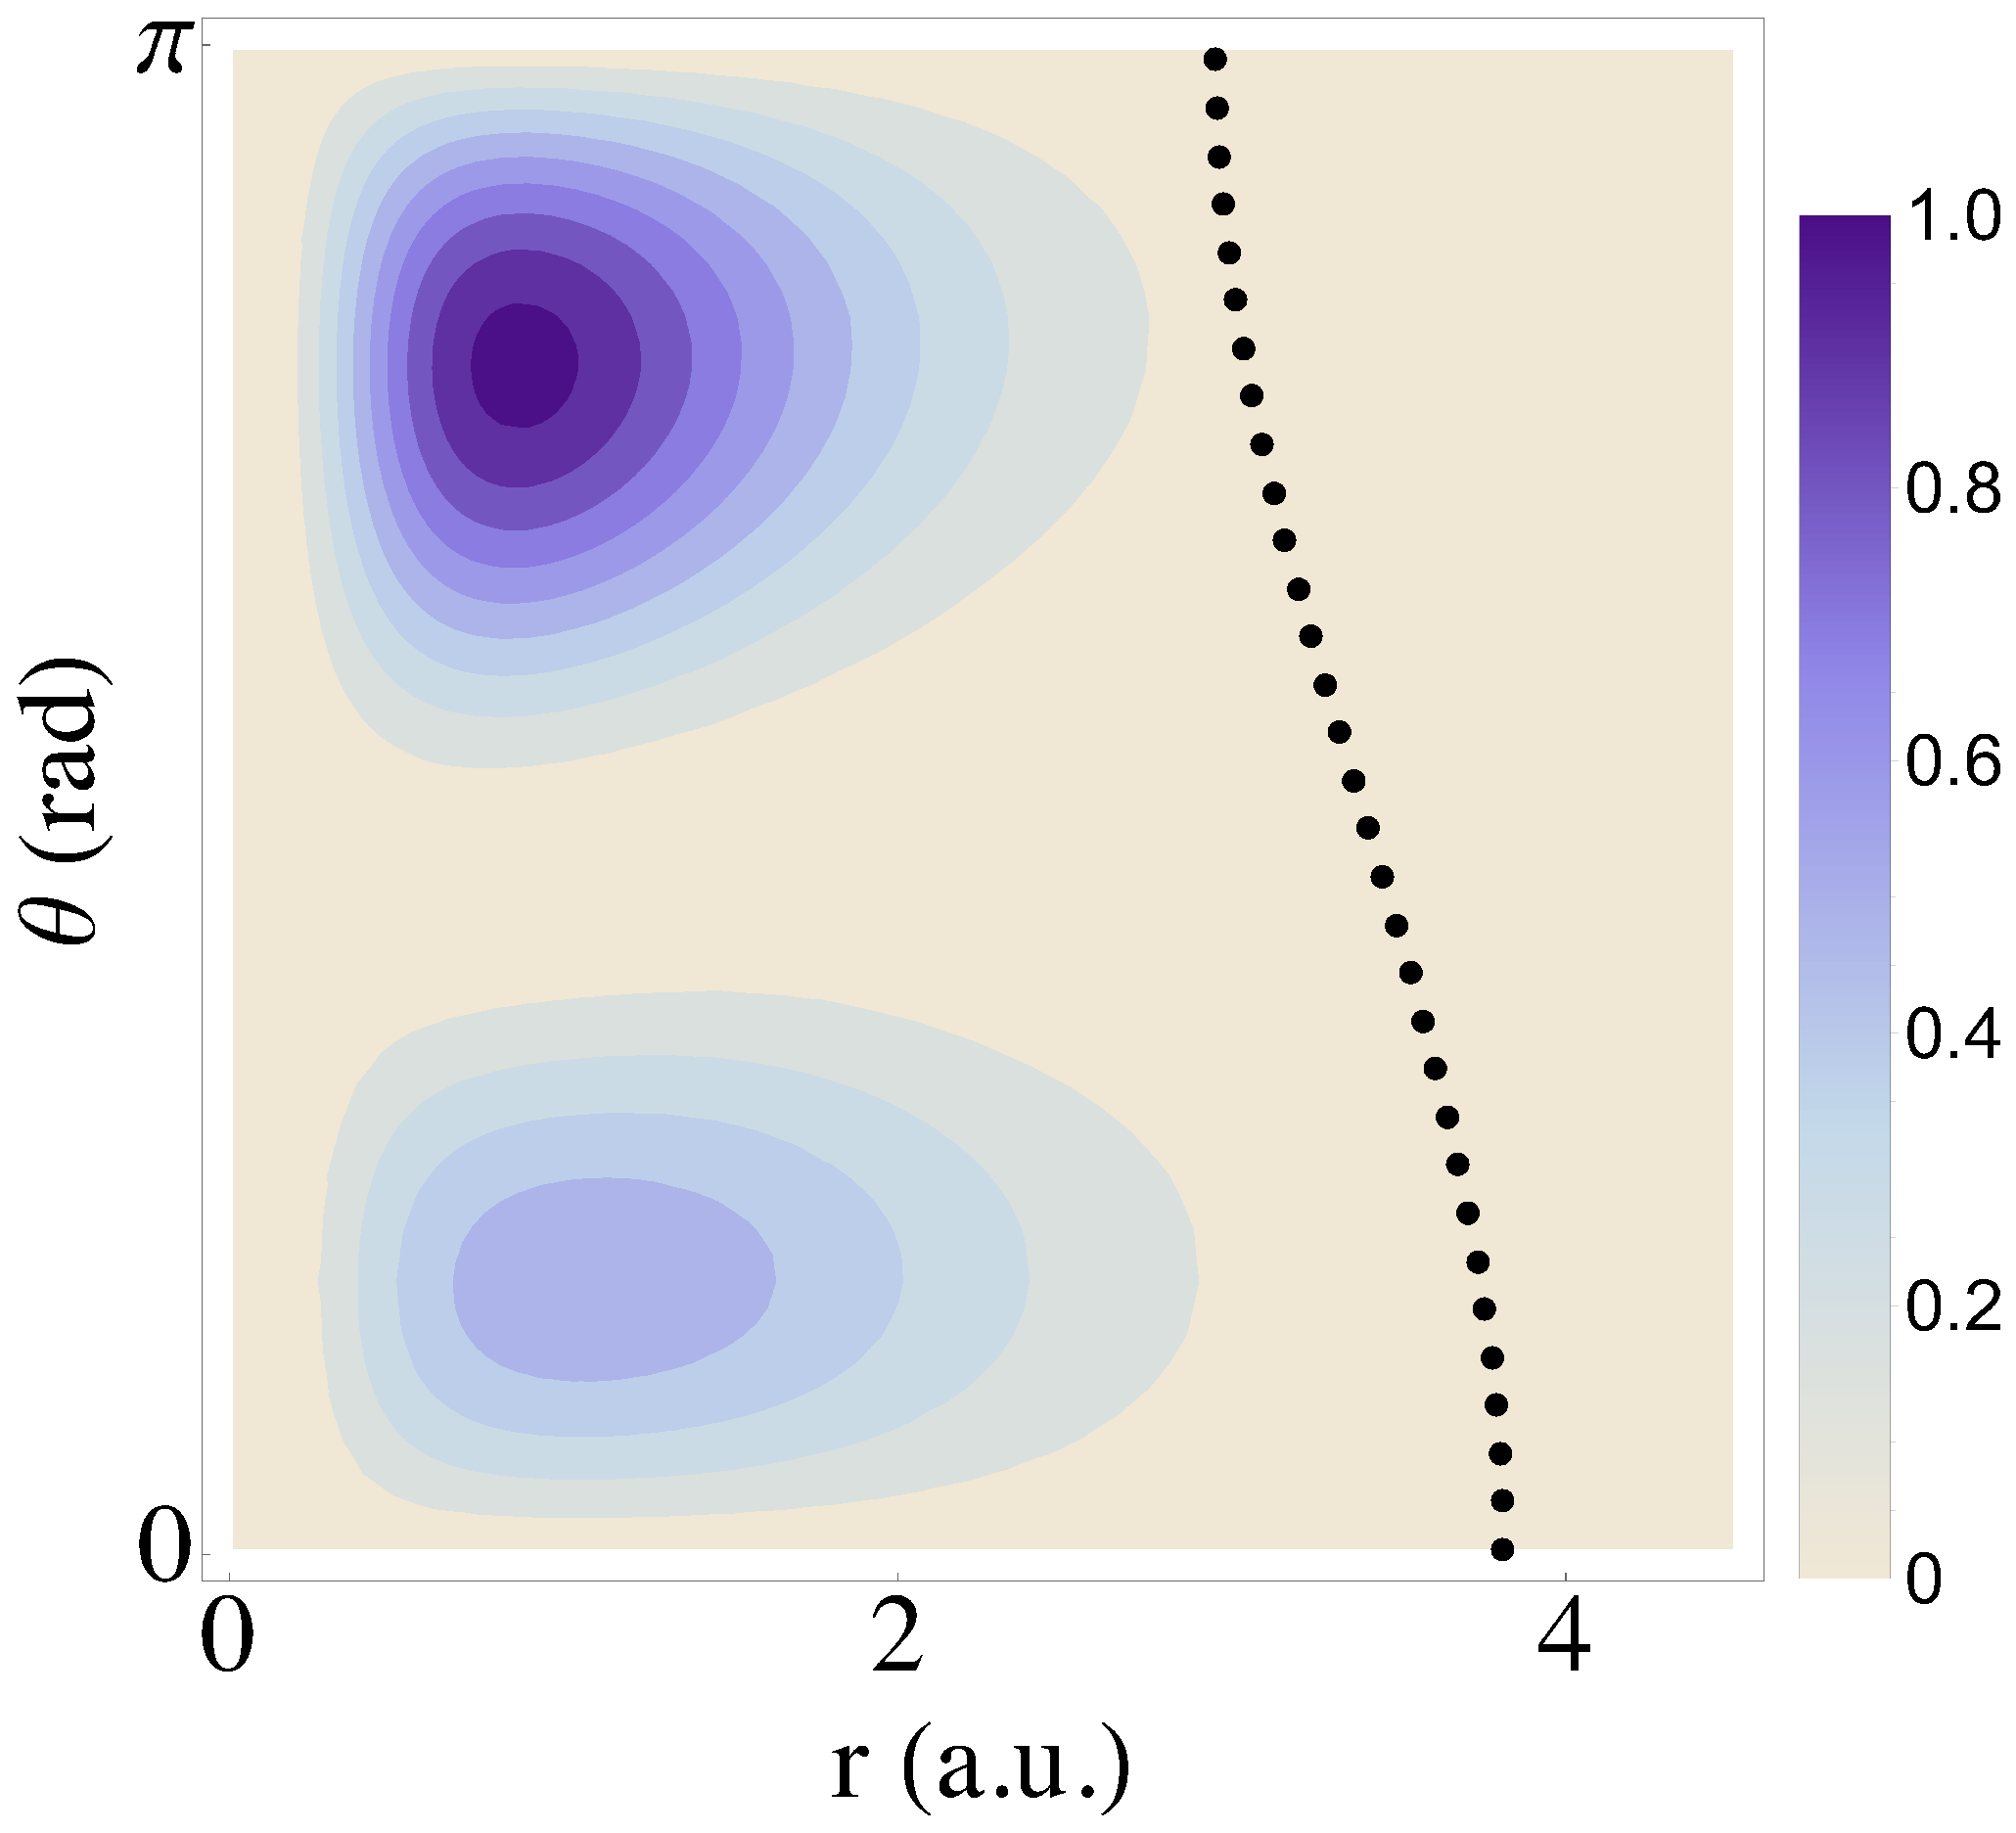
\includegraphics[width=\textwidth]{figures/ch_H2O/3a1/contour3a1intpl.eps}
    \caption{}\label{fig:intp32s}
  \end{subfigure}
  \caption{Contour plots of the scaled probability density,
    $|\psi_{\mathrm{3a_{1}}}|^{2}r^{2}\sin(\theta)/(2\pi)$, for the
    $3a_{1}$ molecular orbital. The orbital density constructed from
    the reduced \textsc{sto} expansion is shown
    in~(\ref{fig:Moccia32s}), while the solution obtained from the
    non-spherical $V_{\mathrm{eff}}(r,\theta)$ with Latter correction
    is shown in~(\ref{fig:intp32s}) along with a dotted line
    indicating where the Latter correction acts. Starting from the
    innermost contours the contour values are $0.45\dots 0.05$ for the
    upper density lobes and $0.2\dots 0.05$ for the lower density
    lobes, in steps of $0.05$.}
  \label{fig:density_contours}
\end{figure}

The interpolation is achieved by collecting data from the evaluation
of the potential on two sections of the $(r,\theta)$ grid in the
vicinity of the nodal line, where the potential evaluates to finite
values. Then, a numerical interpolation was carried out between those
regions in order to obtain a continuous function,
$V_{\mathrm{eff}}^{\mathrm{intp}}(r,\theta)$, on the two-dimensional
grid. The Latter correction is applied to the interpolated potential
and the effective potential is defined according to~(\ref{eq:rMatch}):
%
\begin{eqnarray}
  V_{\mathrm{eff}}(r,\theta) = \left\{
  \begin{split}
    V_{\mathrm{eff}}^{\mathrm{intp}}(r,\theta)\
    & \mathrm{~for} & r < r_{\mathrm{match}}(\theta) \\
    -1/r\ & \mathrm{~for} &  r > r_{\mathrm{match}}(\theta)
  \end{split}
\right.
\label{eq:latterVeff}
\end{eqnarray}
%

Figure~\ref{fig:Moccia32s} shows the probability density for the
$3a_{1}$ \textsc{mo} as a contour plot in the $r-\theta$ plane as
obtained from the reduced Moccia expansion in
\textsc{sto}s~(\ref{eq:3a1Moccia_expansion}). Figure~\ref{fig:intp32s}
shows the same for the solution of the Schr\"{o}dinger
equation~(\ref{eq:sch_eq3d}) using the interpolated
$V_{\mathrm{eff}}(r,\theta)$, defined in
Equation~(\ref{eq:latterVeff}), with the Latter
correction~\cite{LatterCor_1955} applied in the asymptotic $r-$region.

The effective potential~(\ref{eq:latterVeff}) results in the
probability density shown in Figure~\ref{fig:intp32s} and yields an
orbital energy of $-0.5579\ \mathrm{a.u.}$ for the $3a_{1}$
\textsc{mo}, with a relative change of $0.32\%$ in comparison with the
self-consistent result of Moccia~\cite{Moccia_1964} of
$-0.5561\ \mathrm{a.u.}$.

As Figure~\ref{fig:intp32s} indicates, the implementation of the
Latter correction to the orbital-dependent potential obtained from
Equation~(\ref{eq:sch_eq3d}) introduces a slight re-adjustment of the
density, with a somewhat higher probability density in the region $0 <
\theta < \pi/2$. The probabilities for finding the electron at $\pi/2
< \theta < \pi$ is $66.2\%$ before the Latter correction is applied
(Figure~\ref{fig:Moccia32s}) and becomes $63.5\%$ for the case shown
in Figure~\ref{fig:intp32s}.

\subsection{Exterior complex scaling}
\label{ch:3a1_ecs}

For our aim of computing the resonance parameters that describe the
tunneling process, a modified exterior complex scaling to the radial
coordinates was implemented. As was described in
Sec.~\ref{ch:ecs_1b11b2}, the $r-$coordinate is extended into the
complex plane by the phase function $\chi(r)$,
Eq.~(\ref{eq:ecs_theta}), with $r$ replaced by $r^{*} =
r\exp[i\chi(r)]$. The phase function $\chi(r)$ is chosen to be very
small for $r$ values smaller than the Latter radius $\bar{r}$. It then
turns on from nearly zero to reach an asymptotic value
$\chi_{\mathrm{s}}$ at $r-$values just outside where the Latter
correction is applied, i.e., $r_{\mathrm{s}} >
r_{\mathrm{match}}$. The purpose of using the phase function $\chi(r)$
is to implement \textsc{ecs} in a smooth fashion and avoid having an
$r-$value at which a derivative discontinuity would have to be
applied~\cite{ecsScrinzi}.

A non-Hermitian Hamiltonian results from considering the additional
terms that the modified complex scaling to the radial coordinates
introduces in the Schr\"{o}dinger equation. The complex wave function
is separated into real and imaginary parts, $\psi_{R(I)}$, such that
the problem of describing the ionization regime of the $3a_{1}$
\textsc{mo} under an external dc field applied along the orientation
axis of the orbital is expressed in terms of a system of partial
differential equations for the real and imaginary parts of
$\widetilde{\psi}(r,\theta)$ in spherical polar coordinates given
explicitly as Eq.~(\ref{eq:pde_system}). Schematically, the equations
are extensions of the field-free Schr\"{o}dinger
equation~(\ref{eq:sch_eq3d}) and $\widetilde{\psi}(r,\theta)$
satisfies~\cite{sarias_2017}
%
\begin{eqnarray}
  \begin{split}
    \left[ -\frac{1}{2}\nabla^{2} + V_{\mathrm{eff}}(r, \theta)
      \pm F_{0}z \right] \widetilde{\psi}(r,\theta) = (E_{R} - i\Gamma/2)
    \widetilde{\psi}(r, \theta),
  \end{split}
  \label{eq:sch_tunneling_params}
\end{eqnarray}
%
where $E_{R}$ is the resonance position and $\Gamma$ the
width. Compared to Eq.~(\ref{eq:sch_eq3d}), the Hamiltonian in
Eq.~(\ref{eq:sch_tunneling_params}) contains the interaction with the
external field and complex scaling is responsible for the replacement
$E_{3a_{1}} \to E_{R} - i\Gamma/2$; while $\widetilde{\psi}(r,
\theta)$ remains square integrable.

The domains of $r$ and $\theta$ values are restricted to the intervals
$\epsilon < r < r_{\mathrm{max}}$ and $\eta < \theta < \pi - \eta$,
with typical values $\epsilon = 10^{-2}\ \mathrm{a.u.}$, $\eta =
10^{-2}$, $r_{\mathrm{max}} = 28\ \mathrm{a.u.}$ In the limit of low
field strengths, i.e., $F_{0} = 0.05\ \mathrm{a.u.},
0.06\ \mathrm{a.u.}$, the value of $r_{\mathrm{max}}$ was increased to
$40\ \mathrm{a.u.}$ in order to ensure the outer turning points lie
inside the grid, as the tunneling barrier extends to larger $r$.

The problem of finding a solution of the Schr\"{o}dinger equation for
the $3a_{1}$ \textsc{mo} with contributions of $2s$ and $2p-$type
states requires a set of boundary conditions that describes the
properties of the orbital on the grid. In contrast with the numerical
solutions obtained for the $1b_{1}$ and $1b_{2}$ \textsc{mo}s of
H$_{2}$O~\cite{sarias_2016}, Neumann boundary conditions are
implemented for the angular coordinate $\theta$ in order to obtain an
eigenstate and orbital energy consistent with the variational
results~\cite{Moccia_1964}. This choice of boundary conditions, that
the derivative with respect to $\theta$ vanishes at the limits of the
mesh $(\theta = 0 ~\mathrm{and}~ \theta = \pi)$, leads to solutions
$\psi_{R(I)}(r,\theta)$ with a probability density consistent with the
$\theta-$dependence of the $3a_{1}$ orbital, as shown in
Figure~\ref{fig:density_contours}.



\section{Partial-wave method with a complex absorbing potential}
\label{ch:partial_wave}
% describe method, problem to solve and implementation of the
% formalism

%starting point (Madrid potential) we are using a model potential
%introduced by (Illescas2009) in collision calculations[refs]. describe
%the pontential, what has been used for [refs]

%use a multipole decomposition to expand the hydrogen terms of the
%model potential in terms of partial waves

%solve field-free problem and compare to OPM, model potential

The problem of Stark resonances for the H$_{2}$O molecule is treated
with a partial-wave expansion approach~\cite{marko_partialwave} in
which the starting point involves a three-centre model potential that
was initially introduced to simulate the structure of the water
molecule in a study of ion collisions with water
molecules~\cite{illescas_modelV_2011}, and was later used in numerical
calculations of the \textsc{tdse} for proton-water
collisions~\cite{illescas_2015}. The field-free problem is addressed
as well in a convergence study of the orbital energies for the three
H$_{2}$O valence orbitals, namely $1b_{1}, 1b_{2}$ and $3a_{1}$, in
terms of the partial wave expansion limits. The results are contrasted
with a previous calculation that includes the model potential and
Gaussian-type basis~\cite{illescas_2015}.

The model potential is formulated as a superposition of three
spherical potentials, that represent the oxygen atom, and the two
hydrogen atoms of the water molecule at the equilibrium configuration
determined by \textsc{hf} calculations~\cite{illescas_2015}, it has
the form
%
\begin{eqnarray}
  \begin{split}
    V_{\mathrm{mod}} = & V_{\mathrm{O}}(r) + V_{\mathrm{H}}(r_{1}) 
    + V_{\mathrm{H}}(r_{2}) \\
    V_{\mathrm{O}}(r) = & -\frac{8 - N_{\mathrm{O}}}{r} -
    \frac{N_{\mathrm{O}}}{r}(1 + \alpha_{\mathrm{O}}r) \exp(-2\alpha_{\mathrm{O}}r) \\
    V_{\mathrm{H}}(r_{j}) = & -\frac{1 - N_{\mathrm{H}}}{r_{j}} -
    \frac{N_{\mathrm{H}}}{r_{j}}(1 + \alpha_{\mathrm{H}}r_{j}) \exp(-2\alpha_{\mathrm{H}}r_{j}),
  \end{split}
  \label{eq:model_potential}
\end{eqnarray}
%
where $\alpha_{\mathrm{O}} = 1.602$, $\alpha_{\mathrm{H}} = 0.617$ are
screening parameters, $r_{j}$ indicates the electron position relative
to either proton ($j=1,2$), and the electron density `charge
parameters' were chosen as $N_{\mathrm{O}} = 7.185$ and
$N_{\mathrm{H}} = (9 - N_{\mathrm{O}})/2 = 0.9075$ for three highest
occupied \textsc{mo}s of H$_{2}$O. 

The following anzatz in spherical polar coordinates is introduced for
the wave function
%
\begin{eqnarray}
  \begin{split}
    \psi(r,\theta,\phi) & = & \sum\limits_{l=0}\limits^{l_{\mathrm{max}}}
    \sum\limits_{m=-l}\limits^{l} \frac{u_{lm}(r)}{r}
    Y_{l}^{m}(\theta, \phi),
  \end{split}
  \label{eq:spherical_anzats}
\end{eqnarray}
%
where $Y_{l}^{m}$ represents the complex-valued spherical
harmonics. The numerical problem then consists of obtaining the
$u_{lm}(r)$ solutions by solving coupled ordinary differential
equations.

The partial-wave expansion approach for the hydrogen potentials is
implemented as follows. The potential for one hydrogen atom placed on
the $\hat{z}$ axis with distance $R_{j}$ from the oxygen core, as
indicated in the model potential~(\ref{eq:model_potential}), is
expressed as an expansion in terms of Legendre polynomials, such that
for an axially symmetric $\mathrm{O}-\mathrm{H}$ problem one
has~\cite{marko_partialwave}
%
\begin{eqnarray}
  \begin{split}
    V_{\mathrm{H}}(r_{j}) & \approx & \sum\limits_{\lambda=0}
    \limits^{\lambda_{\mathrm{max}}} V_{\lambda}(r) P_{\lambda}(\cos\theta),
  \end{split}
  \label{eq:Legendre-pols}
\end{eqnarray}
%
where the channel potentials $V_{\lambda}(r)$ are obtained by
projecting $V_{\mathrm{H}}(r_{j})$ onto Legendre polynomials. The
hydrogen atom is then rotated into the position consistent with the
H$_{2}$O geometry using the addition theorem for spherical harmonics
%
\begin{eqnarray}
  \begin{split}
    P_{\lambda}(\cos\theta) & = & \frac{4\pi}{2\lambda + 1}
    \sum\limits_{\mu = -\lambda}\limits^{\lambda} Y_{\lambda}^{\mu}(\hat{r}')
    \bar{Y}_{\lambda}^{\mu}(\hat{r}''),
  \end{split}
  \label{eq:add_sphericalYlm}
\end{eqnarray}
%
where $\cos\theta = \hat{r}'\cdot\hat{r}''$. These transformations
lead to obtain one expansion for each hydrogen atom expressed in
$(r,\theta,\phi)$ coordinates. The orientations defined by $\theta'$
correspond to one half of the opening angle, $52.2\ \mathrm{degrees}$,
for each hydrogen atom, respectively, and the azimuthal angles are
$\phi_{1}'=\pi/2$ and $\phi_{2}'=3\pi/2$ in accordance with the
geometry described in~\cite{Moccia_1964}. As a result, a truncated
potential of the form~\cite{marko_partialwave}
%
\begin{eqnarray}
  \begin{split}
    V_{\mathrm{H}}(r,\theta,\phi) & = & \sum\limits_{\lambda=0}
    \limits^{\lambda_{\mathrm{max}}} \frac{4\pi}{2\lambda + 1} V_{\lambda}(r)
    \sum\limits_{\mu=-\lambda}\limits^{\lambda} Y_{\lambda}^{\mu}(\theta,\phi)
    \bar{Y}_{\lambda}^{\mu}(\theta',\phi_{j})
  \end{split}
  \label{eq:expanded_H_potential}
\end{eqnarray}
%
is obtained for each hydrogen atom. 

% describe how to obtain the structure of the radial equations for the
% field-free problem and how to solve the numerical problem to obtain
% the eigenvalues

The partial-wave model potential that results from inserting the
expansion~(\ref{eq:expanded_H_potential}) into the H$_{2}$O model
potential introduced in~(\ref{eq:model_potential}) leads to a system
of coupled radial equations of the form~\cite{marko_partialwave}
%
\begin{eqnarray}
  \begin{split}
    -\frac{u_{l,m}''(r)}{2} + \frac{l(l + 1)}{2r^{2}} u_{l,m}(r)
    + V_{\mathrm{O}}(r) u_{l,m}(r) + \sum\limits_{l',m'}
    R_{l,m}^{l',m'}(r) u_{l',m'}(r) & = & \varepsilon u_{l,m}(r),
  \end{split}
  \label{eq:radial_u}
\end{eqnarray}
%
in which the matrix elements $R_{l,m}^{l',m'}(r)$ contain the
potentials of the hydrogen atoms as partial-wave expansions, and are
evaluated by means of Gaunt integrals~\cite{marko_partialwave}. The
quantum numbers $l,m$ satisfy $l = 0, \dots, l_{\mathrm{max}}$, and
$-l \leq m \leq l$. The reference frame used in this approach places
the oxygen atom at the origin of coordinates, hence the oxygen
potential in~(\ref{eq:radial_u}), $V_{\mathrm{O}}(r)$, represents the
spherically symmetric potential introduced in the model
potential~(\ref{eq:model_potential}).

Once a partial-wave potential has been generated for each hydrogen
atom one can proceed to calculate the eigenvalues for the field-free
problem. The computation of numerical solutions for the coupled
equations for the different $(l,m)$ channels is carried out using
\emph{Mathematica}'s \textsc{nde}igensystem package, which implements
a finite-element mesh to represent the coupled ordinary differential
equations~(\ref{eq:radial_u}).

% describe the finding of the optimal determinant that gives the sol
% to an n-channel problem
The $n-$channel problem to obtain the energy eigenvalues is addressed
in the following manner: given a set of different initial conditions
and a trial energy value, the system of coupled
equations~(\ref{eq:radial_u}) can generate $n$ independent solutions
that are propagated to a given endpoint at large $r$ where one can
build a determinant of the solutions that is ultimately minimized in
an iterative process to find the optimal combination of solutions that
leads to a zero, or small valued, determinant. Ultimately, one wants
to find the energy eigenvalue associated to the overall solution that
is bound at some outer radius, i.e., that evaluates to zero or a very
small value at large $r$. As the number $l_{\mathrm{max}}$ grows, the
number of $(l,m)$ channels increases noticeably and the problem of
finding a numerical solution to~(\ref{eq:radial_u}) becomes more
sensitive to propagated errors, it is necessary in theses cases to
increase the working precision of the calculations.

%apply a CAP to determine the resonance eigenstates as a result of an
%external dc field

The dc-field ionization problem to determine the Stark resonances for
the H$_{2}$O valence orbitals under an external field applied along
the $\hat{z}$-direction is stated by including the external field
potential $-F_{0}r\cos\theta$ in the radial
equations~(\ref{eq:radial_u}). A quadratic complex absorbing
potential~(\textsc{cap}) of the form
%
\begin{eqnarray}
  V_{\mathrm{CAP}} = \left\{
  \begin{split}
    -i \eta_{c}(r - r_{c})^{2} \ & \mathrm{~when} & r > r_{c} \\
    0 \phantom{i \eta_{c}(r - r_{c})^{2}} \ & \mathrm{~when} &  r < r_{c}
  \end{split}
  \right.
\label{eq:VCAP}
\end{eqnarray}
%
is applied to the system of coupled differential equations in order to
determine the complex eigenvalues that result from the effect of the
external dc field. The Stark problem presents a higher numerical
challenge than the field-free one, in this case we are looking for a
solution in the complex plane and the determinant to be minimized is a
complex number, which implies that the condition of convergence to
zero should be applied to its norm.


% describe what \eta and r_c mean, and how to obtain the eigenvalues
% from there
The radius $r_{c}$ in~(\ref{eq:VCAP}) indicates the beginning of the
region where the \textsc{cap} becomes effective. In order to avoid
oscillating outgoing waves in the numerical solutions, it is a good
practice to turn the \textsc{cap} on at distances where the
partial-wave potential~(\ref{eq:expanded_H_potential}) has reached its
simple asymptotic form. This condition is satisfied for $r > 12$ with
great accuracy. The parameter $\eta_{c}$ indicates the strength of the
\textsc{cap}. Ideally, the parameter $\eta_{c}$ should be a small
number in order to have a small artifact introduced to the system of
equations. However, it is important to keep in mind that when
$\eta_{c}\to 0$ numerical errors may increase. Ultimately, the
artificial term introduced by the \textsc{cap} needs to be removed
from the results in order to obtain the resonance
parameters~\cite{RissMeyer_1993}.

The complex eigenvalues that result from applying the
\textsc{cap}~(\ref{eq:VCAP}) to the system of radial
equations~(\ref{eq:radial_u}) are computed according the following
scheme. For a given field strength, $F_{0}$, a set of complex
eigenvalues is computed for an equidistant mesh of strength
parameters, such that $\eta_{c} = n \times 10^{-3}$ for $n = 20,
\dots, 70$. These results are interpolated to a sixth-order polynomial
as a function of $\eta_{c}$, and then the optimal $\eta$ value is
calculated according to the Riss-Meyer correction
scheme~\cite{RissMeyer_1993}, which is implemented up to second order.

According to the Riss-Meyer scheme~\cite{RissMeyer_1993}, the effects
of the \textsc{cap} can be removed by means of an iterative correction
scheme based on perturbation theory, in which the $n$-th order
corrected energy can be expressed as a truncated Taylor expansion of
the form
%
\begin{eqnarray}
  \begin{split}
    E^{(n)} & = & E^{(n)}(\tilde{\eta}) & =
    E_{\mathrm{fb}}(\tilde{\eta}) +
    \sum\limits_{j=1}\limits^{n}
    \left.
    \frac{(-\tilde{\eta})^{j}}{j!} \frac{d^{j}E_{\mathrm{fb}}}{d\eta^{j}}
    \right|_{\eta=\tilde{\eta}}
  \end{split}
  \label{eq:RM_scheme}
\end{eqnarray}
%
where $E_{\mathrm{fb}}$ stands for the finite-basis trajectory of
eigenvalues obtained on the $\eta-$grid, and $\tilde{\eta}$ is the
optimal value of the \textsc{cap} strength at which the total error of
approximating the exact resonance energy is minimal, $\tilde{\eta}$ is
given by the condition
%
\begin{eqnarray}
  \begin{split}
    \left| \frac{\eta^{n+1}}{(n + 1)!} \frac{d^{n+1} E_{\mathrm{fb}}}{d\eta^{n+1}}
    \right|_{\eta=\tilde{\eta}} & = & \mathrm{min}, ~~~~ n = 0,1,2,3.
  \end{split}
  \label{eq:optimal_eta}
\end{eqnarray}
%
The optimal value for the \textsc{cap} parameter depends on the order
of the correction scheme. The $n$th order Riss-Meyer correction can be
interpreted as removal of the artifact provided by the \textsc{cap} by
$n$th order perturbation theory.

As an illustrative example, the trajectory of complex eigenvalues as a
function of the \textsc{cap} strength for a partial-wave calculation
with $l_{\mathrm{max}}=3$ for the $3a_{1}$ \textsc{mo} is shown in
Figure~\ref{fig:3a1_RMtrajectory} for a field intensity of $F_{0} =
-0.1\ \mathrm{a.u.}$. The blue circles indicate the eigenvalues
corresponding to the range of $\eta$ values $[0.003, \dots, 0.06]$ of
the \textsc{cap} parameter in steps of $\Delta\eta = 10^{-3}$. The
results were obtained using \emph{Mathematica}'s
\textsc{nde}igensystem finite-element solver. The trajectory is smooth
for larger values of $\eta$, but it shows remarkable variation at
small $\eta$ (on the left in Fig.~\ref{fig:3a1_RMtrajectory}), which
illustrates the above mentioned difficulty in solving the
Schr\"{o}dinger equation when $\eta_{c}\to 0$.

The stabilization point $(n = 0)$ is shown as a red cross, and the
complex energy values at the accumulation points for $n = 1, 2$ of the
Riss-Meyer iterative correction scheme~(equations~(\ref{eq:RM_scheme})
and~\ref{eq:optimal_eta})) are shown as green and magenta crosses,
respectively. These $n = 1, 2$ perturbatively corrected energies fall
below the curve and indicate to be in close proximity to one
another. Looking at the trajectory of complex eigenvalues and the
locations of the stabilized value ($n = 0$) as well as the corrected
values to first and second order in perturbation theory ($n = 1, 2$),
it can be noticed that the \textsc{cap} results shown in
Figure~\ref{fig:3a1_RMtrajectory} agree up to three significant
digits, both in resonance position and width.

% what the RM corrections represent
% which complex energy was chosen?


\begin{figure}
  \centering
  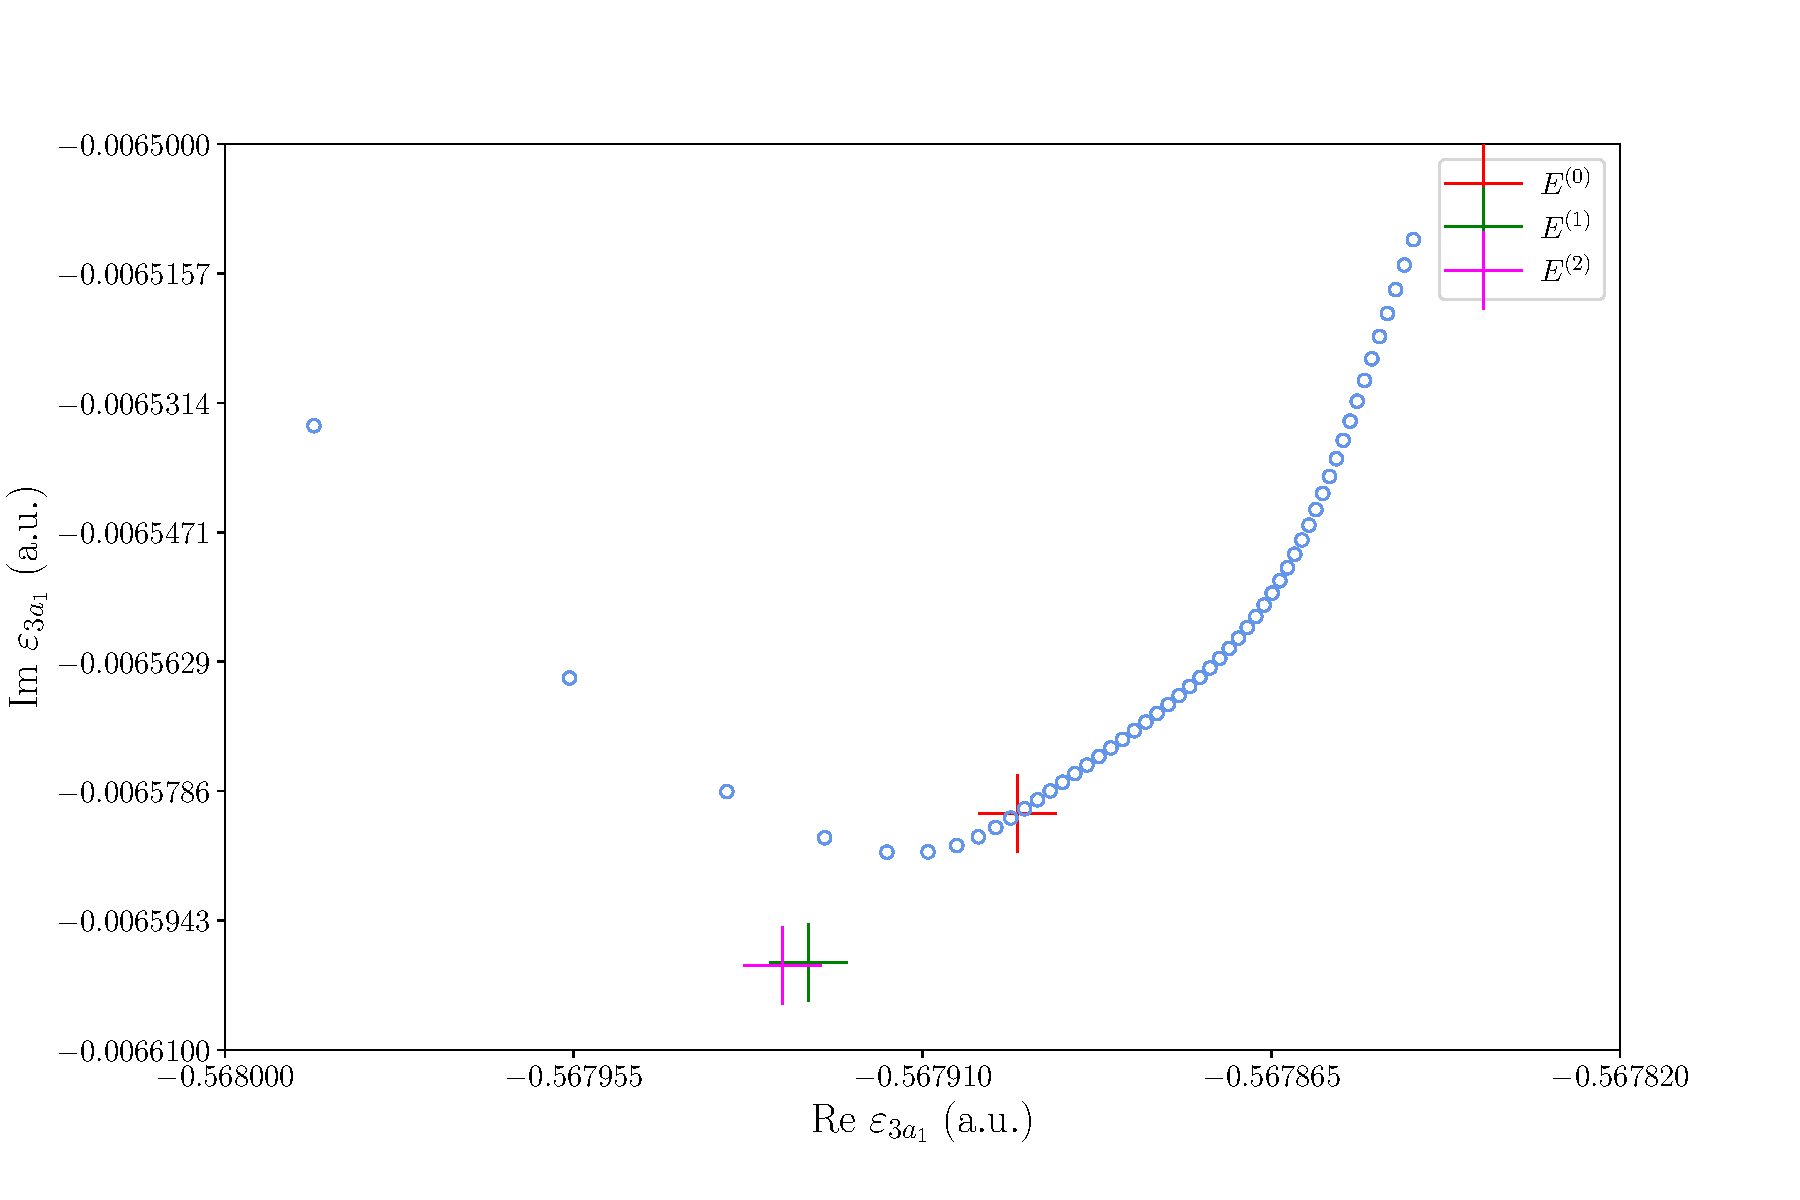
\includegraphics[width=0.85\textwidth]{figures/ch_H2O/partial_wave/3a1trajectory.pdf}
  \caption{Trajectory of complex eigenvalues as a function of
    $\eta_{c}$ (blue circles) corresponding to an $l_{\mathrm{max}}=3$
    calculation of the $3a_{1}$ \textsc{mo}. The energy corresponding
    to the $\eta_{c}$ stabilization value is shown with a red
    cross. The first and second order Riss-Meyer corrected energies
    are indicated as green and magenta crosses, respectively. The
    electric field strength is $-0.1\ \mathrm{a.u.}$}
  \label{fig:3a1_RMtrajectory}
\end{figure}




%determine the complex eigenvalues with a Pade extrapolation and
%Riss-Meyer correction method

%ref to the CAP data from the polynomial expansion as work-in-progress
%(private communication to be published)















% NEXT SECTION
%The physical parameters of interest, namely the resonance position,
%$E_{R}$, and width, $\Gamma = -2E_{I}$, that characterize the
%tunneling process of the quasi-stationary state when an external
%electric dc field is applied along the $\pm\hat{z}$ directions, were
%found by solving the system of partial differential equations
%(Ref.~\cite{PhysRevA.94.053413}) for a set of field strength values,
%$F_{0}$, as if it were an inhomogeneous problem. In the vicinity of a
%location in the $(r,\theta)$ plane where the probability amplitude is
%expected to be large, a two-parameter root search was implemented to
%determine $\{E_{R},E_{I}\}$, the complex energy that maximizes the
%probability density amplitude in the $2d-$grid.



\section{Stark resonance parameters}
\label{ch:stark_params}

Sections~\ref{ch:1b1_1b2_results} and~\ref{ch:3a1_results} present the
numerical results for the physical parameters of interest, namely the
resonance position, $E_{R}$, and width, $\Gamma = -2E_{I}$, that
characterize the tunneling process of the quasi-stationary state when
an external electric dc field is applied along the $\pm\hat{z}$
directions. The system of partial differential
equations~(\ref{eq:pde_system}) is solved for a set of field strength
values, $F_{0}$, as if it were an inhomogeneous problem. In the
vicinity of a location in the $(r,\theta)$ plane in which the
probability amplitude is expected to be large, a two-parameter root
search is implemented in order to determine ${E_{R}, E_{I}}$, the
complex energy that maximizes the probability density amplitude in the
$2d-$grid.

A study of the influence of a set of numerical parameters involved in
the two-dimensional problem~(\ref{eq:pde_system}) on the complex
eigenvalue $E_{R}+iE_{I}$, which describes the ionization process as
an exponential decay in time in terms of resonance position and
half-width, is carried out. In addition to testing the code against
known results for atomic hydrogen~\cite{Telnov_1989}, a systematic
study of the results for the H$_{2}$O valence orbitals against a
number of parameters is performed in order to assess their
accuracy. One parameter concerns the limiting resolution with which
the finite-element method proceeds (the \textsc{maxcellsize} parameter
in the \emph{Mathematica}~10 implementation of \textsc{ndsolve},
denoted as $\Delta$). For values $\Delta < 0.02\ \rm{a.u.}$ we find
stability in the eigenvalues (real and imaginary parts) of two-three
significant digits. For the results quoted in
Secs.~\ref{ch:1b1_1b2_results} and~\ref{ch:3a1_results}, the more
stringent criterion of $\Delta=0.01\ \rm{a.u.}$ is applied.

The second parameter analyzed in this chapter is the range where the
complex scaling function sets in, i.e., $r_{s}$ and $\Delta r$ in
Eq.~(\ref{eq:ecs_theta}). For the scaling method to work the scaling
is required to set in for $r > r_0$, where the effective potential
represents a simple Coulomb tail, which in practice is satisfied by
$r_{s} > 2r_{0}$. Additionally, the condition $\Delta r <
2\ \rm{a.u.}$ is needed to guarantee a smooth turn-on of the scaling
in this region. Small values of $\Delta r$ pose challenges for the
automated finite-element method, since in the limit of $\Delta r \to
0$ one would need to implement the derivative discontinuity in the
solution as discussed by Scrinzi~\cite{ecsScrinzi}. It has been
discussed in the literature that implementing this smooth exterior
scaling of the coordinates into the complex plane is equivalent to
adding a \textsc{cap} to the
Hamiltonian~\cite{ECS_sim_CAP_1991,ECS_sim_CAP_1998}. We find stable
results for the real and imaginary parts of the eigenenergies at the
level of three significant digits for the range $10 < r_{s} <
15\ \rm{a.u.}$ Larger values would require an increase in the
computational domain beyond $r=20\ \rm{a.u.}$

Another systematic that is explored is the choice of the ultimate
scaling angle reached at large $r$, namely the value of
$\chi_{\rm{s}}$ in~(\ref{eq:ecs_theta}). For an accuracy demand of
three significant digits, and the other parameters chosen in the
ranges described above stability in the resonance widths is achieved
for $0.6< \chi_{\rm{s}} < 1.2$ rad.

Finally, Section~\ref{ch:cap_results} discusses the results of the
partial-wave expansion method introduced in Sec.~\ref{ch:partial_wave}
for a model potential that simulates the structure of the H$_{2}$O
molecule~\cite{illescas_modelV_2011}. The partial-wave approach is
combined with a quadratic complex absorbing potential in order to
study the effects of an external dc field. The angular momentum basis
in the model potential expansion is truncated at $l_{\mathrm{max}} =
2$ and $l_{\mathrm{max}} = 3$ including all the associated $m$
values. The resonance positions and widths are obtained from the
complex eigenvalues associated with the non-hermitian analysis of the
system of radial equations~(\ref{eq:radial_u}) introduced by the
\textsc{cap}.


\subsection{$1b_{1}$ and $1b_{2}$ molecular orbitals}
\label{ch:1b1_1b2_results}

% include the plots that the first 3 paragraphs in secIII(PRA2016)
% refer to about the systematic studies of the relevant parameters for
% the calculation

\begin{figure}
  \centering
  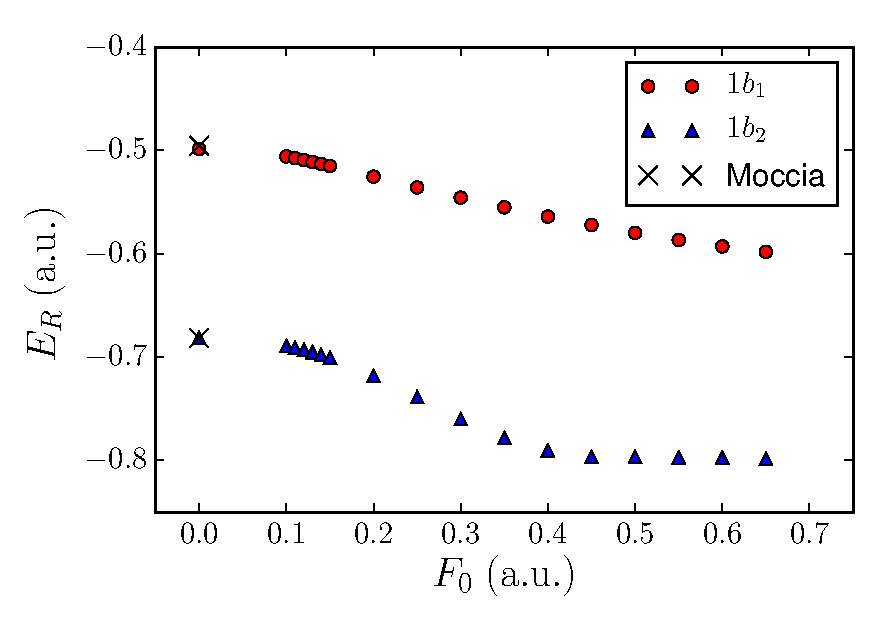
\includegraphics[width=0.7\textwidth]{figures/ch_H2O/1b1_1b2/resPositionvsF1b11b2.eps}
  \caption{Resonance position as a function of the external field
    strength $F_{0}$ for the $1b_{1}$ (red circles) and $1b_{2}$ (blue
    triangles) \textsc{mo}s of H$_{2}$O.}
  \label{fig:1b11b2_position}
\end{figure}

\begin{figure}
  \centering
  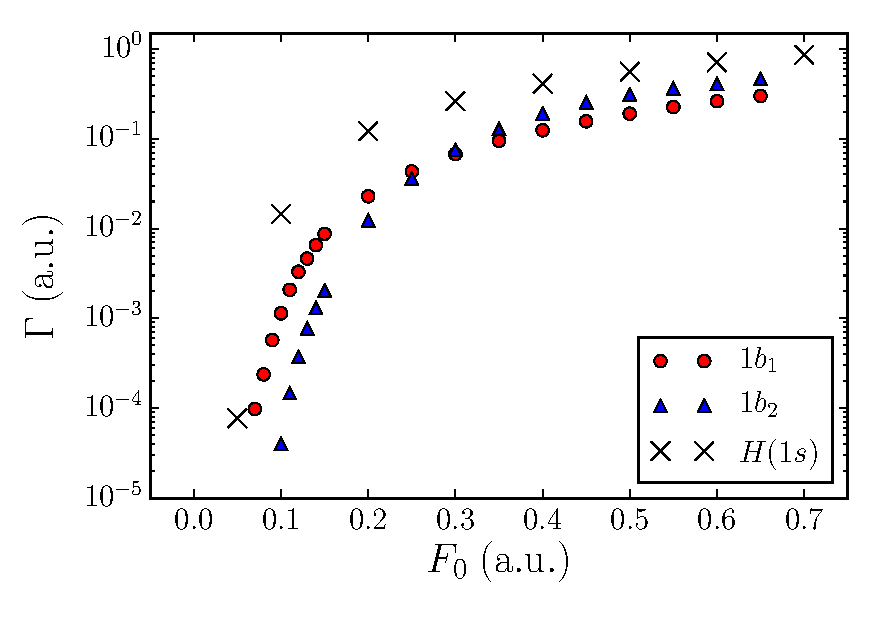
\includegraphics[width=0.7\textwidth]{figures/ch_H2O/1b1_1b2/resWidthvsF1b11b2H1s.eps}
  \caption{Resonance width as a function of the external field
    strength $F_{0}$ for the $1b_{1}$ (red circles) and $1b_{2}$ (blue
    triangles) \textsc{mo}s of H$_{2}$O. For comparison, atomic
    hydrogen H$(1s)$ ionization rates from
    Refs.~\cite{Telnov_1989,Kolosov_1987} are shown as crosses.}
  \label{fig:1b11b2_width}
\end{figure}

Figure~\ref{fig:1b11b2_position} shows the resonance position $E_{R}$
as obtained from the present calculations for the weakly bound
$1b_{1}$ and the strongly bound $1b_{2}$ valence orbitals as a
function of applied electric field strength $F_{0}$. In the limit of
zero field the calculation reproduces the \textsc{scf} eigenvalues of
Moccia~\cite{Moccia_1964}. The field has to be strong (in comparison
with atomic hydrogen results for $2p$ orbitals~\cite{Telnov_1989}) in
order to change the resonance position appreciably. For the more
deeply bound $1b_{2}$ orbital the shift in resonance position
saturates with field strength.

In Figure~\ref{fig:1b11b2_width} the resonance widths are shown for
both orbitals as functions of external field strength $F_{0}$. The
graphs display threshold behavior at the weaker field strengths. As
expected, we find a lower threshold (critical field strength) for the
more weakly bound $1b_{1}$ orbital. Interestingly, however, at a field
strength of about $F_{0} = 0.3\ \mathrm{a.u.}$ the values for the
widths cross; that is, the more deeply bound $1b_{2}$ orbital displays
a larger ionization rate as the field strength is increased further.

Also shown in Figure~\ref{fig:1b11b2_width} are the widths for the
H($1s$) orbital from Refs.~\cite{Telnov_1989,Kolosov_1987}. They can
be compared to the $1b_{1}$ orbital results, since the binding energy
is very close in the free-field limit. Since the tunneling barrier is
mostly in the asymptotic regime where the potential energy has a
$-1/r$ tail, it is not surprising that the widths for
H$_{2}$O($1b_{1}$) and H($1s$) share some similarity in shape. In the
tunneling region H($1s$) has an ionization rate that is larger by
about an order of magnitude. In the over-barrier regime, however, the
ionization rates approach each other to within a factor of 3. Reasons
for why the $1b_1$ water molecular orbital is harder to ionize than
H($1s$) have to do with the different shape of the orbital density
($m=1$ \emph{vs} the spherical H($1s$) density), and the substantially
more attractive potential at shorter distances.

An examination of contour plots of the densities $\Psi^{*}\Psi$, as
well as of the potential energies $V_{\mathrm{eff}} - F_{0}z$ for
different field strengths (both as a function of $r,\theta$), allows
us to make the following observations. For field strengths $F_{0} <
0.1\ \mathrm{a.u.}$ there is a barrier the electrons need to penetrate
in order to be ionized. From the potential-energy plot shown in
Figure~\ref{fig:1b11b2_position} one can see that for weak fields
(small values of $F_{0}$) the barrier is longer for the more deeply
bound $1b_{2}$ orbital. This explains why the ionization threshold
occurs for $F_{0} > 0.1\ \mathrm{a.u.}$ for this orbital, which is
about a factor of $2$ larger than for the $1b_{1}$ orbital.

The field-strength region where the ionization rates (resonance
widths) display a change in character, i.e., turn over to rise much
more gradually with the field strength $F_{0}$, can be characterized
as a regime where there is a narrow potential saddle at small $\theta$
in the vicinity of $r \approx 3\ \mathrm{a.u.}$, such that electron
flux can leave and is then accelerated by the electric field. The
crossing of the ionization rates for the $1b_{1}$ and $1b_{2}$
orbitals occurs since the saddle in the potential becomes effectively
lower at strong fields for the $1b_{2}$ orbital. This can be inferred
from the comparison of the two effective potentials, which share the
same asymptotic behaviour beyond $r = 4.3\ \mathrm{a.u.}$ (see
Figure~\ref{fig:Veff1b11b2}).

The origin for the different radial dependencies of the effective
potential for the two orbitals can be found in the geometry of the
water molecule. The weakly bound $1b_{1}$ orbital has its lobes
perpendicular to the plane defined by the location of the three
nuclei. Therefore, it is least affected by the two protons. The
$1b_{2}$ orbital explores the potentials due to the protons more
strongly in the \textsc{scf} calculation of Moccia, and therefore, the
resulting $V_{\mathrm{eff}}(r)$ has a more attractive region in the
range $0.7\ \mathrm{a.u.} < r < 4.3\ \mathrm{a.u.}$.

%The numerical results are summarized in Table~\ref{tab:1b11b2_results}
%for further reference, i.e., for future comparisons with calculations
%based on other models for the molecular orbitals.

%\begin{table}[t]
%\centering
%\caption{\label{tab:1b11b2_results} Resonance positions and widths for
%  different field strengths (in atomic units). The numbers in
%  parentheses indicate the exponent $k$; that is, the numbers are to
%  be multiplied by $10^{k}$.}
%\begin{tabular}{rrrrr}
%\toprule
% & & $1b_{1}$ & & $1b_{2}$ \\
%$F_{0}$ & $E_{R}$ & $\Gamma$ & $E_{R}$ & $\Gamma$ \\
%\midrule
%$0.1$ & $-0.506$ & $1.14(-3)$ & $-0.689$ & $4.04(-5)$ \\
%$0.2$ & $-0.525$ & $2.28(-2)$ & $-0.718$ & $1.23(-2)$ \\
%$0.3$ & $-0.546$ & $6.74(-2)$ & $-0.760$ & $7.51(-2)$ \\
%$0.4$ & $-0.564$ & $1.24(-1)$ & $-0.790$ & $1.91(-1)$ \\
%$0.5$ & $-0.580$ & $1.90(-1)$ & $-0.796$ & $3.11(-1)$ \\
%$0.6$ & $-0.593$ & $2.61(-1)$ & $-0.797$ & $4.11(-1)$ \\
%\bottomrule
%\end{tabular}
%\end{table}


\subsection{$3a_{1}$ molecular orbital}
\label{ch:3a1_results}

The numerical results from applying the procedure described in
Section~\ref{ch:3a1} are shown in Figures~\ref{fig:3a1_position}
and~\ref{fig:3a1_width}.

\begin{figure}
  \centering
  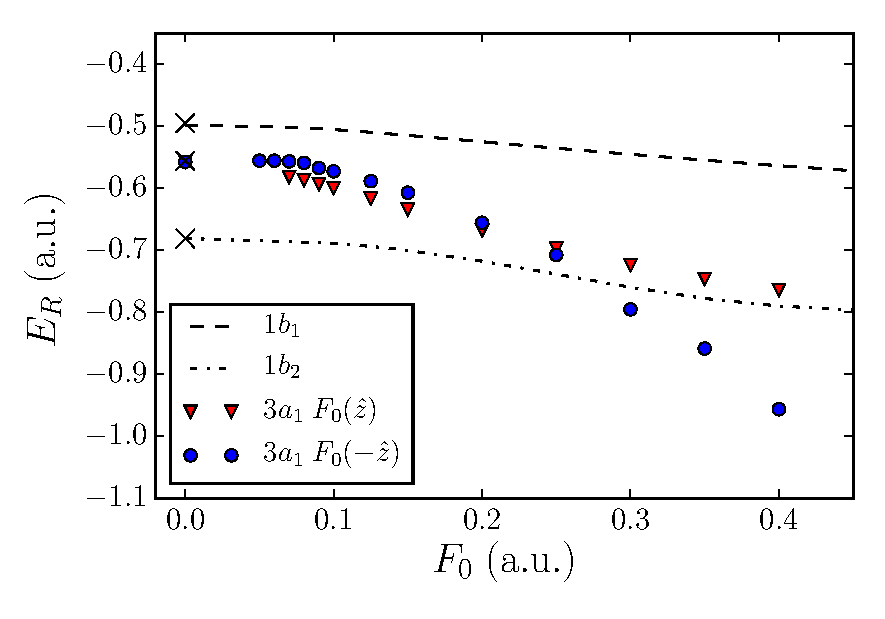
\includegraphics[width=0.7\textwidth]{figures/ch_H2O/3a1/resPosvsForbitals_compf32snew.eps}
  \caption{Resonance position in atomic units as a function of the
    external field strength $F_{0}$ and the orientation of the field,
    along the $\pm\hat{z}$ direction (red triangles/blue circles), for
    the $3a_{1}$ \textsc{mo} of H$_{2}$O. As a reference, the resonance
    position values for the $1b_{1}$ (dashed line) and $1b_{2}$
    (dot-dashed line) \textsc{mo}s are also included.}
  \label{fig:3a1_position}
\end{figure}

\begin{figure}
  \centering
  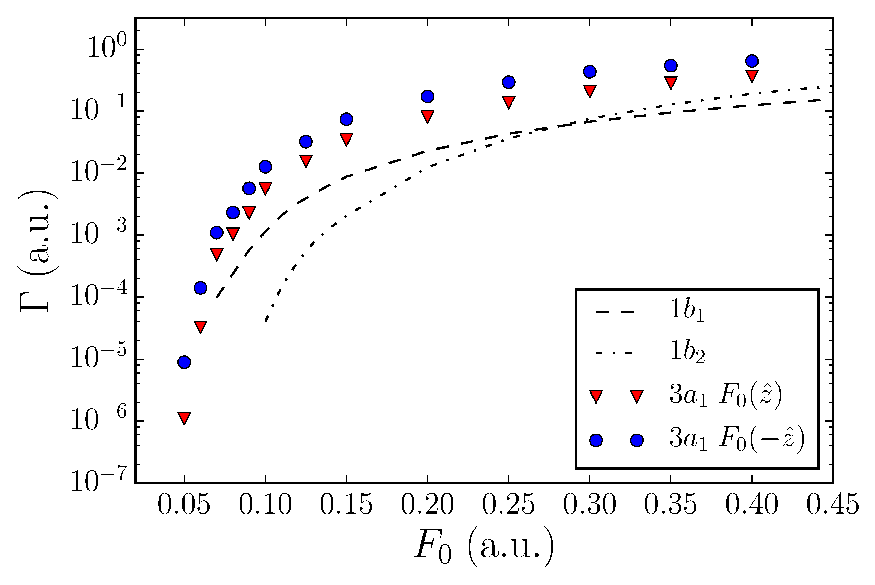
\includegraphics[width=0.7\textwidth]{figures/ch_H2O/3a1/resWidthvsForbitals_compf32snew.eps}
  \caption{Resonance width in atomic units as a function of the
    external field strength $F_{0}$ and the orientation of the field,
    along the $\pm\hat{z}$ direction (red triangles/blue circles), for
    the $3a_{1}$ \textsc{mo} of H$_{2}$O. For reference, the resonance
    widths for the $1b_{1}$ (dashed line) and $1b_{2}$ (dot-dashed
    line) \textsc{mo}s are also shown.}
  \label{fig:3a1_width}
\end{figure}

The resonance positions $E_{R}$ are shown in
Figure~\ref{fig:3a1_position} for external fields applied along the
$\pm\hat{z}$ directions (red triangles/blue circles) for a range of
external field strengths. For reference, the resonance positions
obtained for the $1b_{1}$ and $1b_{2}$ \textsc{mo}s using a
spherically symmetric potential, $V_{\mathrm{eff}}(r)$, are also
indicated in the form of dashed and dot-dashed lines respectively. For
zero field strength $F_{0} = 0$ self-consistent eigenenergies obtained
by Moccia~\cite{Moccia_1964} are included as black crosses for the
three valence orbitals of interest. The resonance position for the
$3a_{1}$ orbital is bracketed by those for the $1b_{1}$ and $1b_{2}$
orbitals.

It can be noticed that for external fields applied along the
$-\hat{z}$ direction, where most of the density is located, the field
strength $F_{0}$ has to be strong, i.e., $F_{0}>0.1\ \mathrm{a.u.}$,
for the resonance position to change appreciably. On the other hand,
the resonance position for fields applied along $+\hat{z}$ appears to
be more sensitive at weaker fields. However the barrier appears to be
longer for external fields applied along the $+\hat{z}$ direction, at
a field strength of about $F_{0} = 0.2\ \mathrm{a.u.}$ the position
values cross, indicating a higher sensitivity of the resonance
positions for fields applied along the negative $\hat{z}$ direction as
the field strength is increased further.

Figure~\ref{fig:3a1_width} shows the resonance widths corresponding to
external fields applied along the $\pm\hat{z}$ directions, as a
function of the field strength $F_{0}$. The results obtained with a
symmetric effective potential, $V_{\mathrm{eff}}(r)$, for the $1b_{1}$
and $1b_{2}$ \textsc{mo}s are also shown as dashed and dot-dashed
lines for comparison purposes.

In analogy to the $1b_{1}$ and $1b_{2}$ orbitals, the ionization rates
for the $3a_{1}$ \textsc{mo}, associated with the lifetime of the
decaying state via $\Gamma\tau=1$, exhibit a threshold behaviour at
the weaker field strengths. Interestingly, for the two directions of
the applied field, we find a lower critical field strength for the
$3a_{1}$ orbital in comparison to what the more weakly bound orbital,
$1b_{1}$, indicates.  In the tunneling region, the $3a_{1}$ orbital
for fields applied along the $-\hat{z}$ direction (blue squares) shows
an ionization rate that is about one order of magnitude larger than
the ionization rate for fields applied in the opposite direction (red
triangles), this gap becomes narrower as the field strength increases
toward the over-barrier regime.

The numerical results for the H$_{2}$O valence orbitals studied in
this chapter, $1b_{1}$, $1b_{2}$ and $3a_{1}$, are summarized in
Table~\ref{tab:3a1_results} for further reference, i.e., to allow
comparison with future calculations based on other models for the
molecular orbitals.


\begin{table}[t]
\centering
\caption{\label{tab:3a1_results} Resonance positions and widths for
  different field strengths (in atomic units). The orientation of the
  external field is indicated by $\pm\hat{z}$. The numbers in
  parentheses indicate the exponent $k$, so that the numbers are
  multiplied by $10^{k}$.}
\begin{tabular}{rrrrrrrrr}
\toprule
&& $3a_{1}(\hat{z})$ && $3a_{1}(-\hat{z})$ && $1b_{1}$ && $1b_{2}$ \\
\midrule
$F_{0}$&$E_{R}$&$\Gamma$&$E_{R}$&$\Gamma$&$E_{R}$&$\Gamma$&$E_{R}$&$\Gamma$ \\
\midrule
$0.05$ &   --~~ &$1.09(-6)$&$-0.556$&$8.91(-6)$ & --~~ & --~~ & --~~ & --~~ \\
$0.06$ &   --~~ &$3.23(-5)$&$-0.556$&$1.41(-4)$ & --~~ & --~~ & --~~ & --~~ \\
$0.07$ &$-0.582$&$4.82(-4)$&$-0.557$&$1.09(-3)$&$-0.502$&$9.82(-5)$ & --~~ & --~~ \\
$0.08$ &$-0.587$&$1.03(-3)$&$-0.559$&$2.31(-3)$&$-0.503$&$2.38(-4)$ & --~~ & --~~ \\
$0.09$ &$-0.594$&$2.26(-3)$&$-0.568$&$5.65(-3)$&$-0.504$&$5.72(-4)$ & --~~ & --~~ \\
$0.1$  &$-0.600$&$5.53(-3)$&$-0.573$&$1.26(-2)$&$-0.506$&$1.14(-3)$&$-0.689$&$4.04(-5)$\\
$0.125$&$-0.617$&$1.54(-2)$&$-0.589$&$3.21(-2)$&$-0.510$&$3.76(-3)$&$-0.694$&$5.45(-4)$\\
$0.15$ &$-0.635$&$3.41(-2)$&$-0.607$&$7.39(-2)$&$-0.515$&$8.73(-3)$&$-0.701$&$2.04(-3)$\\
$0.2$  &$-0.668$&$7.98(-2)$&$-0.656$&$1.72(-1)$&$-0.525$&$2.28(-2)$&$-0.718$&$1.23(-2)$\\
$0.25$ &$-0.698$&$1.37(-1)$&$-0.708$&$2.92(-1)$&$-0.536$&$4.33(-2)$&$-0.739$&$3.61(-2)$\\
$0.3$  &$-0.724$&$2.07(-1)$&$-0.796$&$4.31(-1)$&$-0.546$&$6.74(-2)$&$-0.760$&$7.51(-2)$\\
$0.35$ &$-0.747$&$2.81(-1)$&$-0.859$&$5.40(-1)$&$-0.555$&$9.46(-2)$&$-0.778$&$1.27(-1)$\\
$0.4$  &$-0.765$&$3.60(-1)$&$-0.957$&$6.40(-1)$&$-0.564$&$1.24(-1)$&$-0.790$&$1.91(-1)$\\
\bottomrule
\end{tabular}
\end{table}

\subsection{Ionization parameters from a partial-wave approach}
\label{ch:cap_results}

Figure~\ref{fig:energies_fieldfree} shows the convergence of the three
H$_{2}$O valence \textsc{mo} eigenvalues as a function of the basis
size parameter $l_{\mathrm{max}}$. The comparison with the orbital
energies obtained previously using the model potential with a Gaussian
basis in a quantum chemistry program~\cite{illescas_2015} (shown as
solid lines) reveals that the outermost orbital, $1b_{1}$, with its
density perpendicular to the molecular plane, converges rapidly,
because the density has limited overlap with the hydrogen atoms, as
indicated in Fig.~\ref{fig:h2o_1b1_1b2}. The calculated orbital
energies fall slightly below the quoted values in
Ref.~\cite{illescas_2015}. The values indicated as dash-dotted lines
correspond to a local self-consistent potential approach, namely the
optimized potential method~(\textsc{opm})~\cite{opm_2007}. The
\textsc{opm} represents a Hartree-Fock equivalent calculation in which
an effective local potential is optimized by means of a variational
method to yield self-consistent results that correspond to minimizing
the total energy. The \textsc{opm} total energy and outermost orbital
energy are comparable with Hartree-Fock results. The \textsc{opm}
values quoted in Fig.~\ref{fig:energies_fieldfree} are an interesting
comparison point since they result from an effective self-consistent
potential.

The $1b_{1}$ orbital is referred to as the highest occupied molecular
orbital, and the Koopman's theorem in \textsc{hf}
theory~\cite{Koopman_th_2018} can be carried over to density
functional theory~(\textsc{dft}) methods which have a correct
asymptotic form of the effective potential and has been investigated
for molecules~\cite{HF_molecules_2010}. The experimental ionization
energies of water can be deduced from photoelectron spectroscopy, but
they are complicated by vibrational level structures and are
significantly broadened; quoted values for the three valence orbitals
correspond to ionization energies of $0.68, 0.54, 0.46$ for $1b_{2},
3a_{1}, 1b_{1}$, respectively~\cite{2020Photoelectron}.

For the $3a_{1}$ orbital, which contributes to the bonding of the
water molecule the convergence with $l_{\mathrm{max}}$ is not as
fast. One can expect therefore more interesting phenomena from the
Stark resonance parameter calculations for this case. Convergence with
$l_{\mathrm{max}}$ is really slow for the bonding orbital $1b_{2}$ due
to the fact that a considerable amount of electron density appears
along each O-H bond.

\begin{figure}
  \centering
  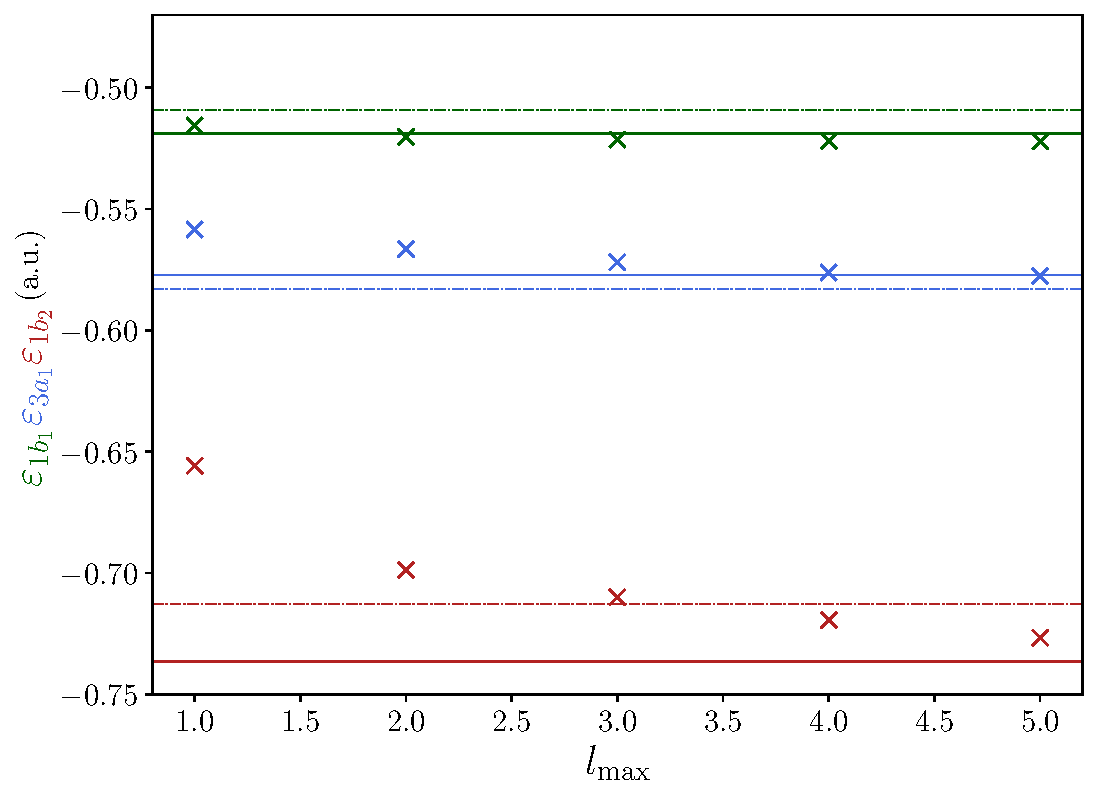
\includegraphics[width=0.85\textwidth]{figures/ch_H2O/partial_wave/eigenvalues_fieldfree.pdf}
  \caption{Eigenvalues for the H$_{2}$O valence molecular orbitals
    $1b_{1}, 3a_{1}, 1b_{2}$ obtained from the model
    potential~(\ref{eq:model_potential}) as a function of the basis
    truncation parameter $l_{\mathrm{max}}$ are shown in green, blue
    and red, respectively. The eigenvalues obtained for the model
    potential as quoted in Ref.~\cite{illescas_2015} are shown as
    solid lines. Also as a reference, the eigenvalues for an
    exchange-only density functional theory approximation
    (\textsc{opm}) from Ref.~\cite{opm_2007} are shown as dash-dotted
    lines.}
  \label{fig:energies_fieldfree}
\end{figure}

The results of complex eigenenergies for the outermost \textsc{mo}
$1b_{1}$ are shown in Fig.~\ref{fig:1b1_cap} for $l_{\mathrm{max}} =
2,3$ as blue and red crosses, respectively. As a comparison the
results obtained from the one-centre expansion local potential
combined with a modified \textsc{ecs} are indicated as purple
crosses. The left panel indicates the real part of the eigenvalue as
the resonance position, and the right panel shows the imaginary part,
which represents the resonance width. When the electric field is
pointing towards the oxygen atom, $F_{z} < 0$, the electrons are
pushed towards the protons, which lowers their eigenenergy
considerably (binding is represented by the magnitude of the real
part). When the electric field is pointing away from the oxygen,
$F_{z} > 0$, the electrons are attracted towards the nucleus, which
initially decrease in binding, but eventually the attraction to the
oxygen reinforces their binding as the field strength increases.

The resonance width shown in the right panel indicates that there is a
strong dependence on the field strength at weak fields where the
tunneling regime dominates. Where there is a marked increase in the
exponential decay rate. As the field strength increases in both
directions one observes a turnover towards the over-barrier ionization
regime. For $F_{z} < 0$, the continuous lowering of the orbital
energies observed in the left panel is accompanied by an increase in
the decay rate that exceeds the rate observed in the opposite
direction by about a factor of two in the over-barrier ionization
regime.




\begin{figure}
  \centering
  \begin{subfigure}[b]{0.45\linewidth}
    \centering
    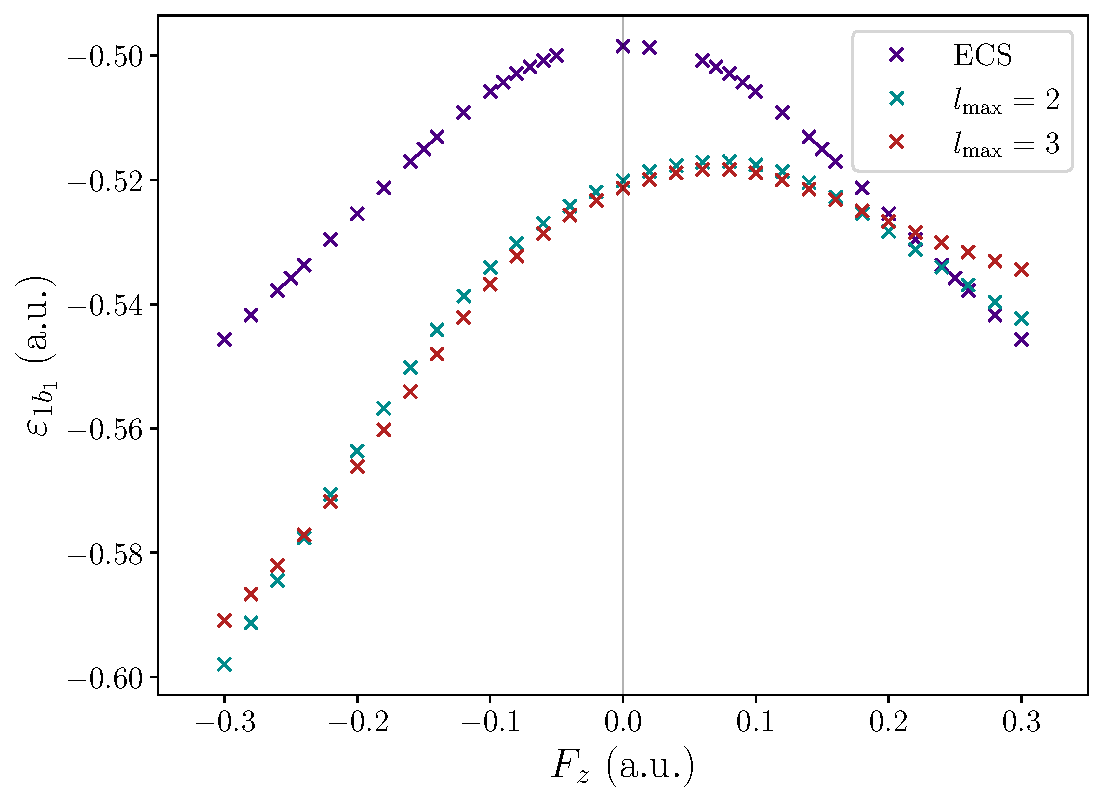
\includegraphics[width=\textwidth]{figures/ch_H2O/partial_wave/Re1b1l23.pdf}
    \caption{}\label{fig:1b1_cap_re}
  \end{subfigure}
  \,
  \begin{subfigure}[b]{0.45\linewidth}
    \centering
    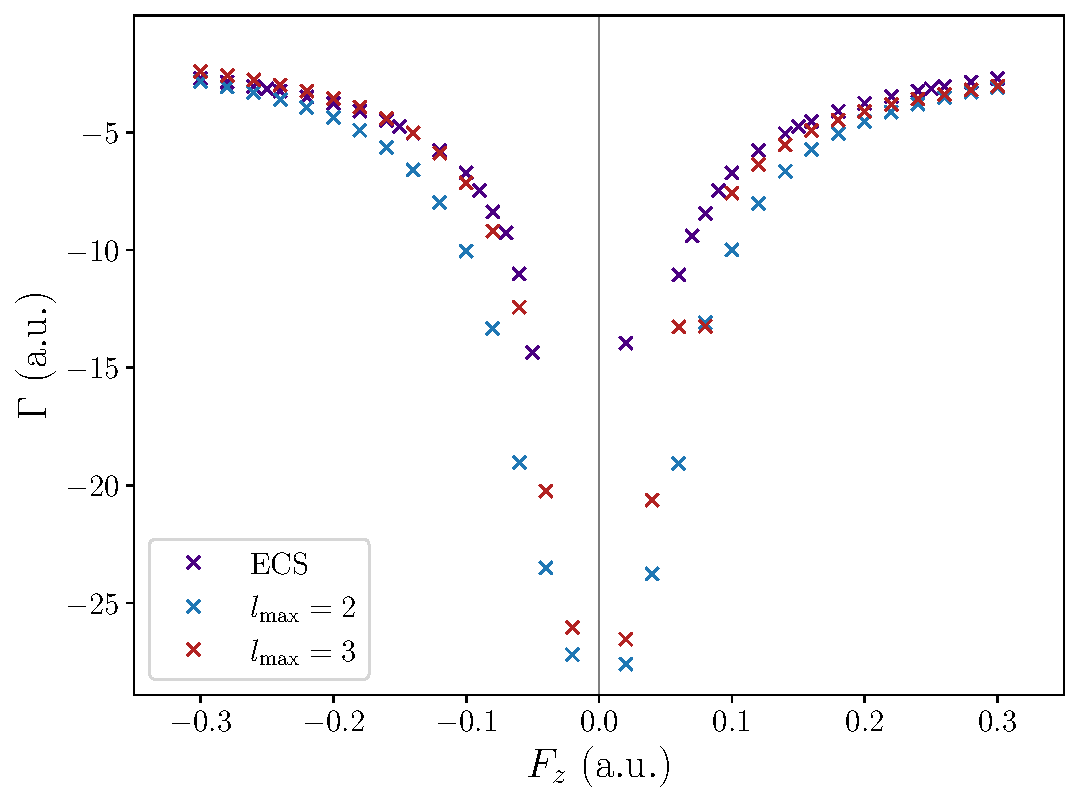
\includegraphics[width=\textwidth]{figures/ch_H2O/partial_wave/Im1b1l23.pdf}
    \caption{}\label{fig:1b1_cap_im}
  \end{subfigure}
  \caption{Resonance parameters for the $1b_{1}$ \textsc{mo} of
    H$_{2}$O. The results for the truncation parameter
    $l_{\mathrm{max}} = 2, 3$ are shown as blue and red crosses,
    respectively. The results obtained with a modified \textsc{ecs}
    are shown as purple crosses. The electric field is pointing in the
    molecular plane from the oxygen atom along a centre line between
    the two hydrogen atoms (for $F_{z} > 0$), and towards the oxygen
    atom (for $F_{z} < 0$).}
  \label{fig:1b1_cap}
\end{figure}

The complex eigenenergies for the partial-wave-\textsc{cap} approach
corresponding to the $1b_{2}$ \textsc{mo} are shown in
Fig.~\ref{fig:1b2_cap}. In this case, convergence with the truncation
parameter $l_{\mathrm{max}}$ is slower than for the $1b_{1}$ valence
orbital. This is consistent with the behaviour observed in
Fig.~\ref{fig:energies_fieldfree} for the field-free case. The
$1b_{2}$ orbital, which is the most deeply bound of the three valence
orbitals, is harder to ionize as can be noticed in the widths that
reach about one half of those for the $1b_{1}$ \textsc{mo} at strong
fields in either direction respectively (see
Fig.~\ref{fig:1b2_cap_im}). These decay rates also indicate that for
the given field range the tunneling regime is dominant. As was
observed for the $1b_{1}$ \textsc{mo}, when the electric field points
towards the oxygen atom, $F_{z} < 0$, the $1b_{2}$ is easier to ionize
than in the opposite direction.


% COMBINE THIS PARAGRAPH WITH COMPARISON WITH PREVIOUS RESULTS FOR 1B1
% AS WELL, AS THE TRENDS ARE SIMILAR

% CONTRAST THE RESULTS FROM THE ONE-CENTRE MODEL POTENTIAL USED WITH A
% MODIFIED ECS, HOW THEY ARE SYMMETRIC WITH RESPECT TO FIELD
% DIRECTION, FAILING TO SHOW OTHER FEATURES

Concerning the \textsc{ecs} results, shown as purple crosses in
Figs.~\ref{fig:1b1_cap} and~\ref{fig:1b2_cap}, derived from a local
effective potential corresponding to a one-centre expansion with an
\textsc{sto} basis~\cite{sarias_2016}, some remarkable features
require a discussion. The resonance positions in the left panels show
a symmetric behaviour about $F_{z} = 0$. This contrasts the
partial-wave-\textsc{cap} calculations which are more sensitive to the
orientation of the external field showing a more pronounced dc shift
for both the $1b_{1}$ and $1b_{2}$ \textsc{mo}s, respectively. On the
other hand, comparable results are observed in the decay rates as a
function of the field orientation and strength shown in the right
panels.

\begin{figure}
  \centering
  \begin{subfigure}[b]{0.45\linewidth}
    \centering
    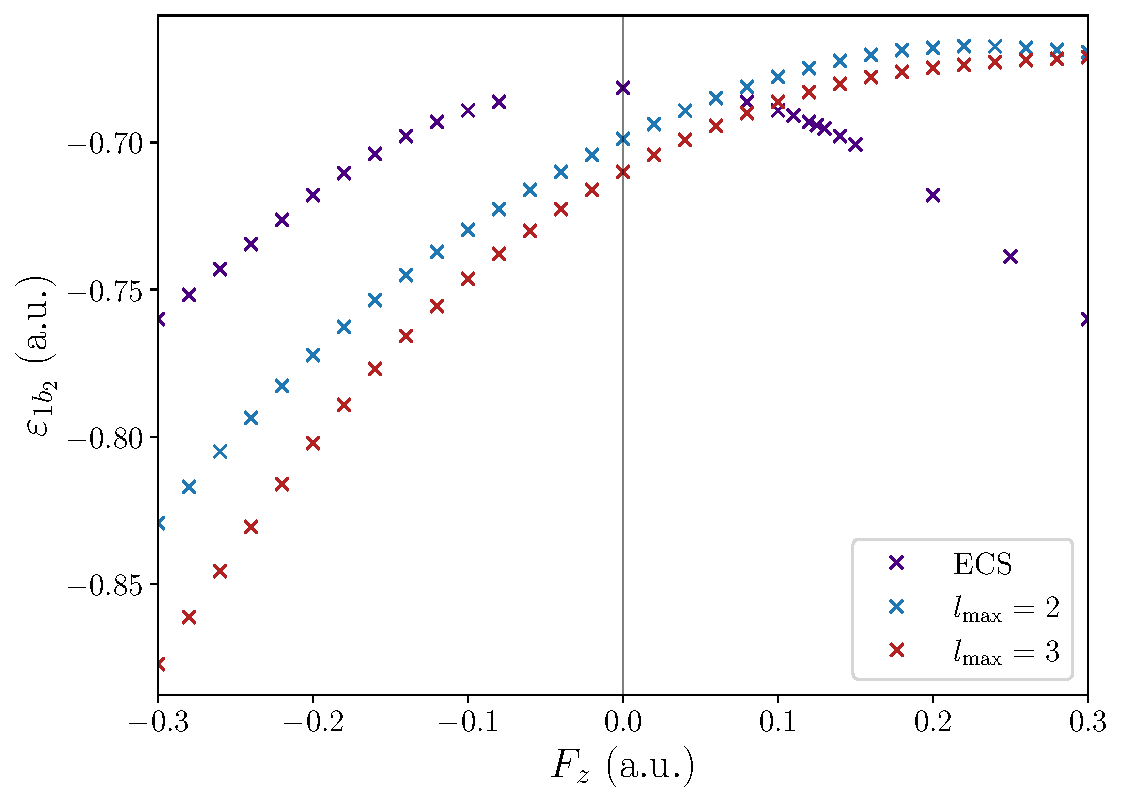
\includegraphics[width=\textwidth]{figures/ch_H2O/partial_wave/Re1b2l23.pdf}
    \caption{}\label{fig:1b2_cap_re}
  \end{subfigure}
  \,
  \begin{subfigure}[b]{0.45\linewidth}
    \centering
    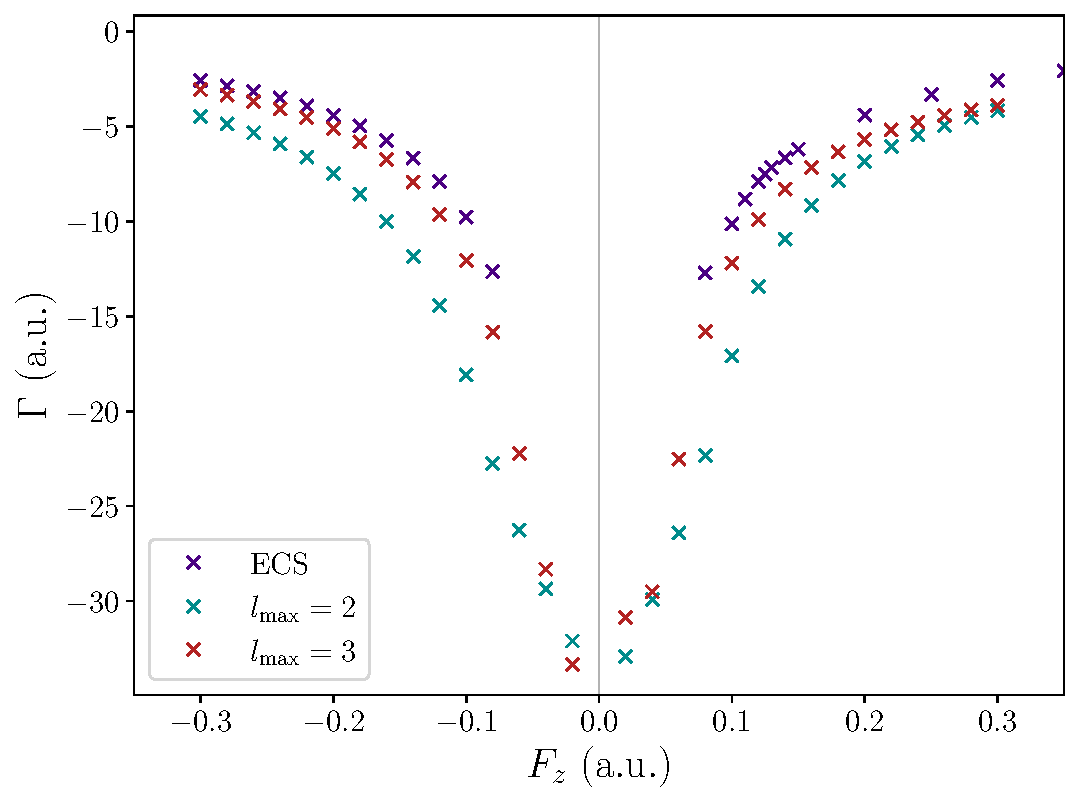
\includegraphics[width=\textwidth]{figures/ch_H2O/partial_wave/Im1b2l23.pdf}
    \caption{}\label{fig:1b2_cap_im}
  \end{subfigure}
  \caption{Resonance parameters for the $1b_{2}$ \textsc{mo} of
    H$_{2}$O. The results for the truncation parameter
    $l_{\mathrm{max}} = 2, 3$ are shown as blue and red crosses,
    respectively. The results obtained with a modified \textsc{ecs}
    are shown as purple crosses. The electric field is pointing in the
    molecular plane from the oxygen atom along a centre line between
    the two hydrogen atoms (for $F_{z} > 0$), and towards the oxygen
    atom (for $F_{z} < 0$).}
  \label{fig:1b2_cap}
\end{figure}

The partial-wave results for the $3a_{1}$ valence orbital are shown in
Figure~\ref{fig:3a1_cap}. The $3a_{1}$ \textsc{mo}, with a probability
distribution along the $\hat{z}$-direction on the molecular plane
formed by the three nuclei, presents remarkable results that follow a
unique trend. In contrast with the monotonic increase in binding that
is observed in Figs.~\ref{fig:1b1_cap} and~\ref{fig:1b2_cap} when the
electric field is pointing towards the oxygen atom ($F_{z} < 0$), the
resonance position (Fig.~\ref{fig:3a1_cap_re}) exhibits a different
pattern as the external field pushes the electrons towards the
hydrogen atoms. Two oscillating trends are observed, corresponding to
each orientation of the dc field. A similar feature was reported for
molecular Stark shift calculations based on the total energy of the
H$_{2}$O molecule~\cite{Jagau_manybody_H2O}.


% comparison with previous calculations with single-centre SCF
% effective potential
Comparing these results with the previous calculations based on a
single-centre \textsc{scf} effective potential~\cite{sarias_2017},
indicated as purple crosses in Fig.~\ref{fig:3a1_cap}, it can be
noticed that the partial-wave expansion of a model potential provides
a more sensitive solution that preserves distinctive features of the
Stark dc shift and decay rate. Some agreement in the resonance
positions can be noticed at low field strengths on each side of the
$F_{z}$ axis. This could be attributed to the extension of the
\textsc{scf} effective potential to include a polar angle dependence
for the $3a_{1}$ orbital (see Eq.~(\ref{eq:latterVeff}) for the
effective potential $V_{\mathrm{eff}}(r,\theta)$), as opposed to the
$1b_{1}$ and $1b_{2}$ orbitals. However, the inclusion of the
dependence in this effective potential on the azimuthal angle $\phi$
seems crucial in order to reproduce the behaviour observed for the dc
Stark shift.

As Fig.~\ref{fig:3a1_cap_im} indicates, the resonance widths from
previous results are similar to the widths obtained with the
partial-wave-\textsc{cap} approach, with the decay rate diverging for
the case where electrons are pushed away from the oxygen atom towards
the two protons by about a factor of two at $F_{z} =
-0.3\ \mathrm{a.u.}$


\begin{figure}
  \centering
  \begin{subfigure}[b]{0.45\linewidth}
    \centering
    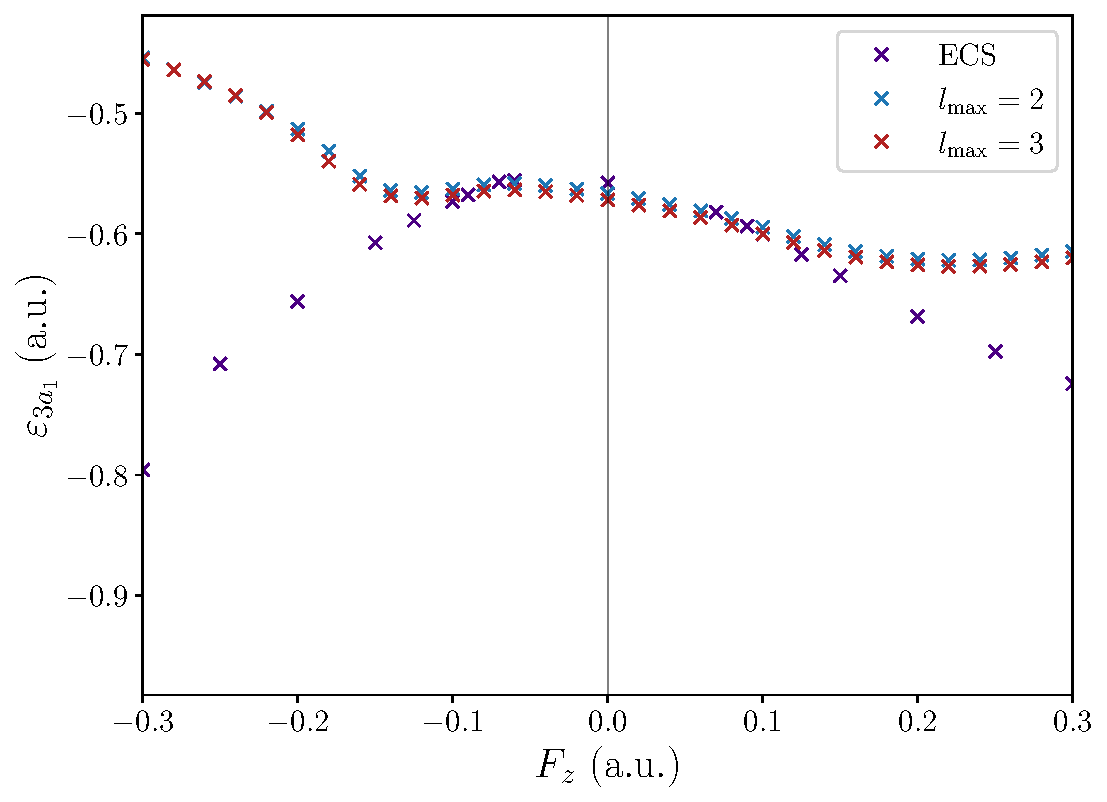
\includegraphics[width=\textwidth]{figures/ch_H2O/partial_wave/Re3a1l23.pdf}
    \caption{}\label{fig:3a1_cap_re}
  \end{subfigure}
  \,
  \begin{subfigure}[b]{0.45\linewidth}
    \centering
    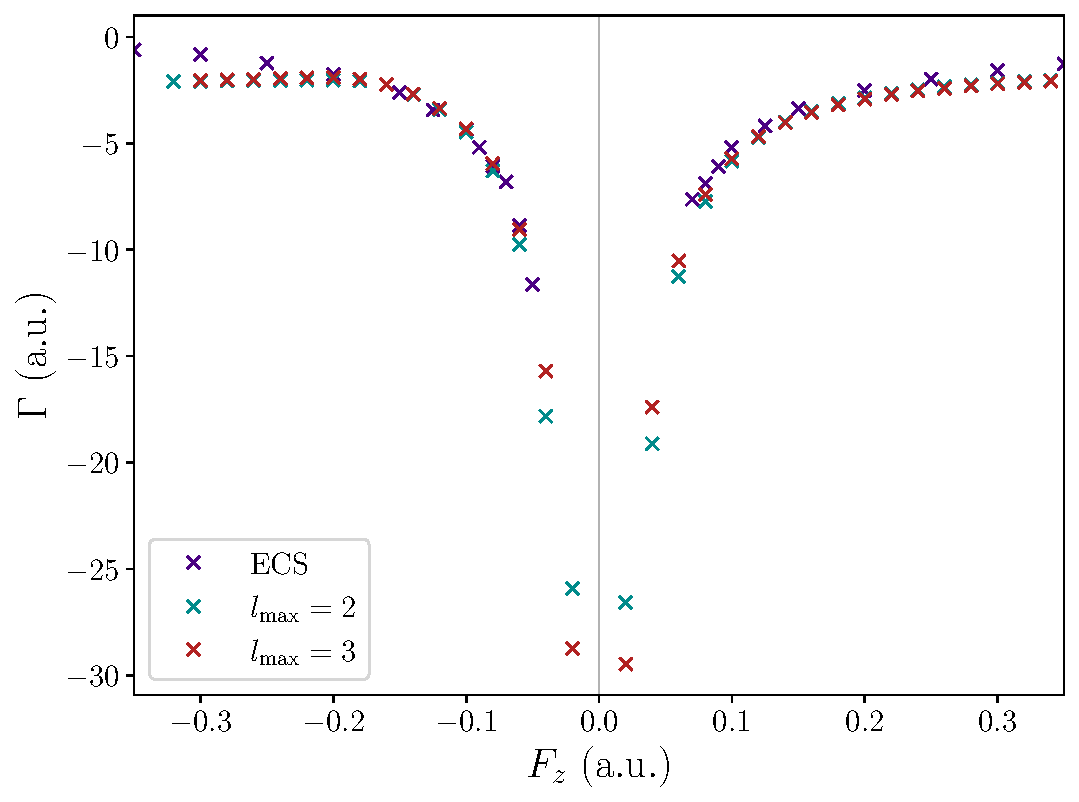
\includegraphics[width=\textwidth]{figures/ch_H2O/partial_wave/Im3a1l23.pdf}
    \caption{}\label{fig:3a1_cap_im}
  \end{subfigure}
  \caption{Resonance parameters for the $3a_{1}$ \textsc{mo} of
    H$_{2}$O. The results for the truncation parameter
    $l_{\mathrm{max}} = 2, 3$ are shown as blue and red crosses,
    respectively. The results obtained with a modified \textsc{ecs}
    are shown as purple crosses. The electric field is pointing in the
    molecular plane from the oxygen atom along a centre line between
    the two hydrogen atoms (for $F_{z} > 0$), and towards the oxygen
    atom (for $F_{z} < 0$).}
  \label{fig:3a1_cap}
\end{figure}





%%% Local Variables:
%%% mode: latex
%%% TeX-master: "thesis"
%%% End:
